\documentclass[12pt,oneside]{sotsuken_paper}

% タイトル
\title{安全な教育用マルチコプターの開発}
\author{北山天斗・剱崎健太郎}

\begin{document}
% 行間
\setlength{\baselineskip}{9truemm}

% 文字間
\kanjiskip=.53zw plus 3pt minus 3pt
\xkanjiskip=.53zw plus 3pt minus 3pt

% 目次
\tableofcontents
%\newpage

% 本文

\chapter{はじめに}

\section{研究背景}
当研究室では例年,機械の制御について研究を行っている.
今年度は近年様々な分野で注目されいているマルチコプターを使って何かやってみたいと考えた.
そこで私達は教育機関に所属している者なので機械制御について学ぶ上で役に立つものをつくろうと考えた.

\section{研究目的}
今年度以降の研究や授業を円滑に進めることができるようにする.
プロペラに巻き込まれて怪我をする事故事例があるため,機体を球形カバーで覆うなど安全化を行う.
以上のことを考え,以下の3つの目標を掲げた.

\begin{itemize}
	\item 機体の製作マニュアルを作成
	\item RaspberryPiでの制御実習環境の構築
	\item 機体を球形カバーで覆う
\end{itemize}

\section{本論文の構成}
本論文の構成は以下の通りである.
第2章では機体,球体などのハードウェアについて,第3章ではソフトウェアについて述べる.


\chapter{ハードウェア}

\section{目標}
強度や重量,製作費,メンテナンス性などを考慮し開発を行う.
また,機体の保護,安全化を目的とし機体を覆う球体カバーの開発を行う.

\section{仕様}
開発したマルチコプターの機体,球体についてそれぞれの仕様を以下に示す.
また,実際に製作したマルチコプターを図\ref{fig:multicopter}に示す.

\begin{figure}[htbp]
	\begin{center}
		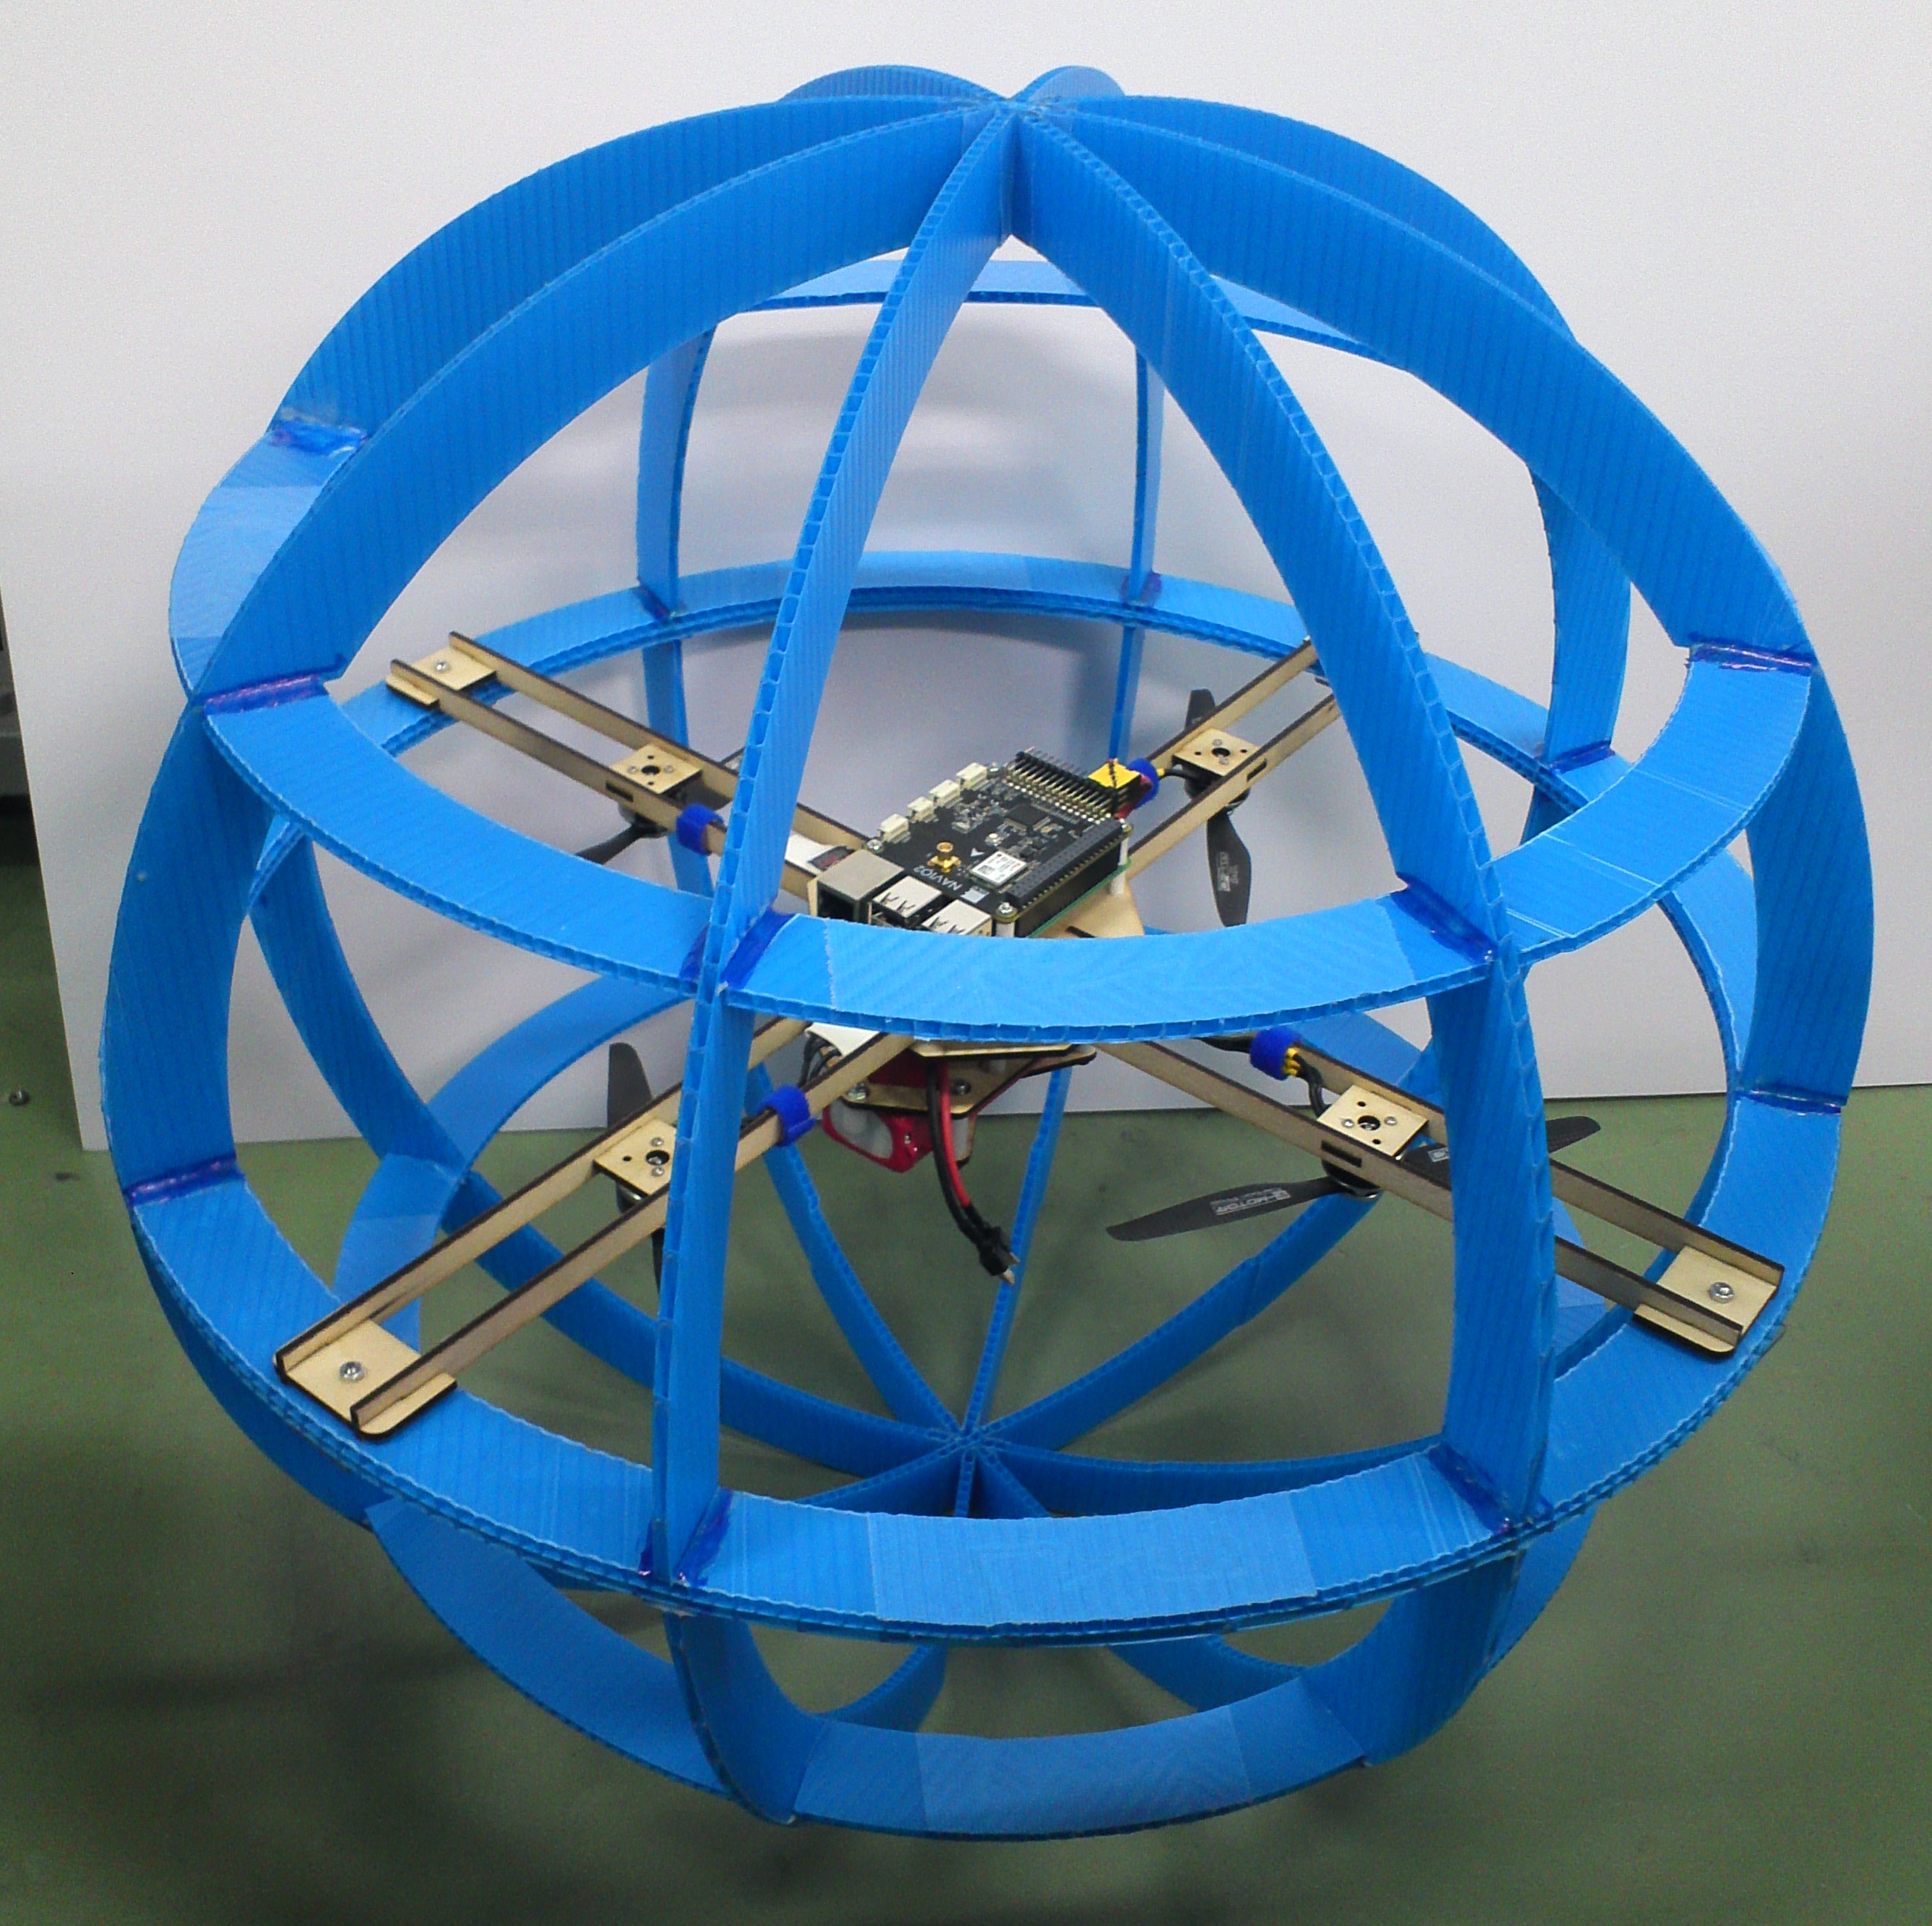
\includegraphics[width=60mm]{image/multicopter.jpg}
		\caption{製作したマルチコプター}
		\label{fig:multicopter}
	\end{center}
\end{figure}

\subsection{機体}
厚さ3mmの木の板から切り出したパーツを主に使用している.
アームの長さは前後左右ともに500mm,プロペラの中心間距離は275mm,高さは100mm,重量は476gとなっている.
T-MOTOR製のモータMN1804,モータドライバ(ESC)S12A,プロペラP6x2prop-2PCS/PAIRを使用している.
バッテリーは11.1v,2200mAhのKT2200-3S-35Cを使用している.
特徴としてモータが機体下部に設置されている.

\subsection{球体}
厚さ4mmのポリプロピレン製プラスチックダンボールの環を木組み構造を用いて直径510mmの骨組み球体に組み上げている.
この球体は上下2つの半球に分解できるようになっている.
重量は223gである.

\section{開発の経緯}
機体,球体についてそれぞれの開発の経緯を以下に示す.

\subsection{機体}

\subsubsection{1号機}
1号機では厚さ2mmのアルミ板,80mm×80mm,厚さ2mmのアルミ角管を主に使用している.
また,RaspberryPiの取付板として120mm×120mm,厚さ1mmのCFRPの板を使用している.
実際に製作した試作1号機を図\ref{fig:drone-1}に示す.
この機体ではアームの強度やバッテリーの取付方法などが問題となった.

\begin{figure}[htbp]
	\begin{center}
		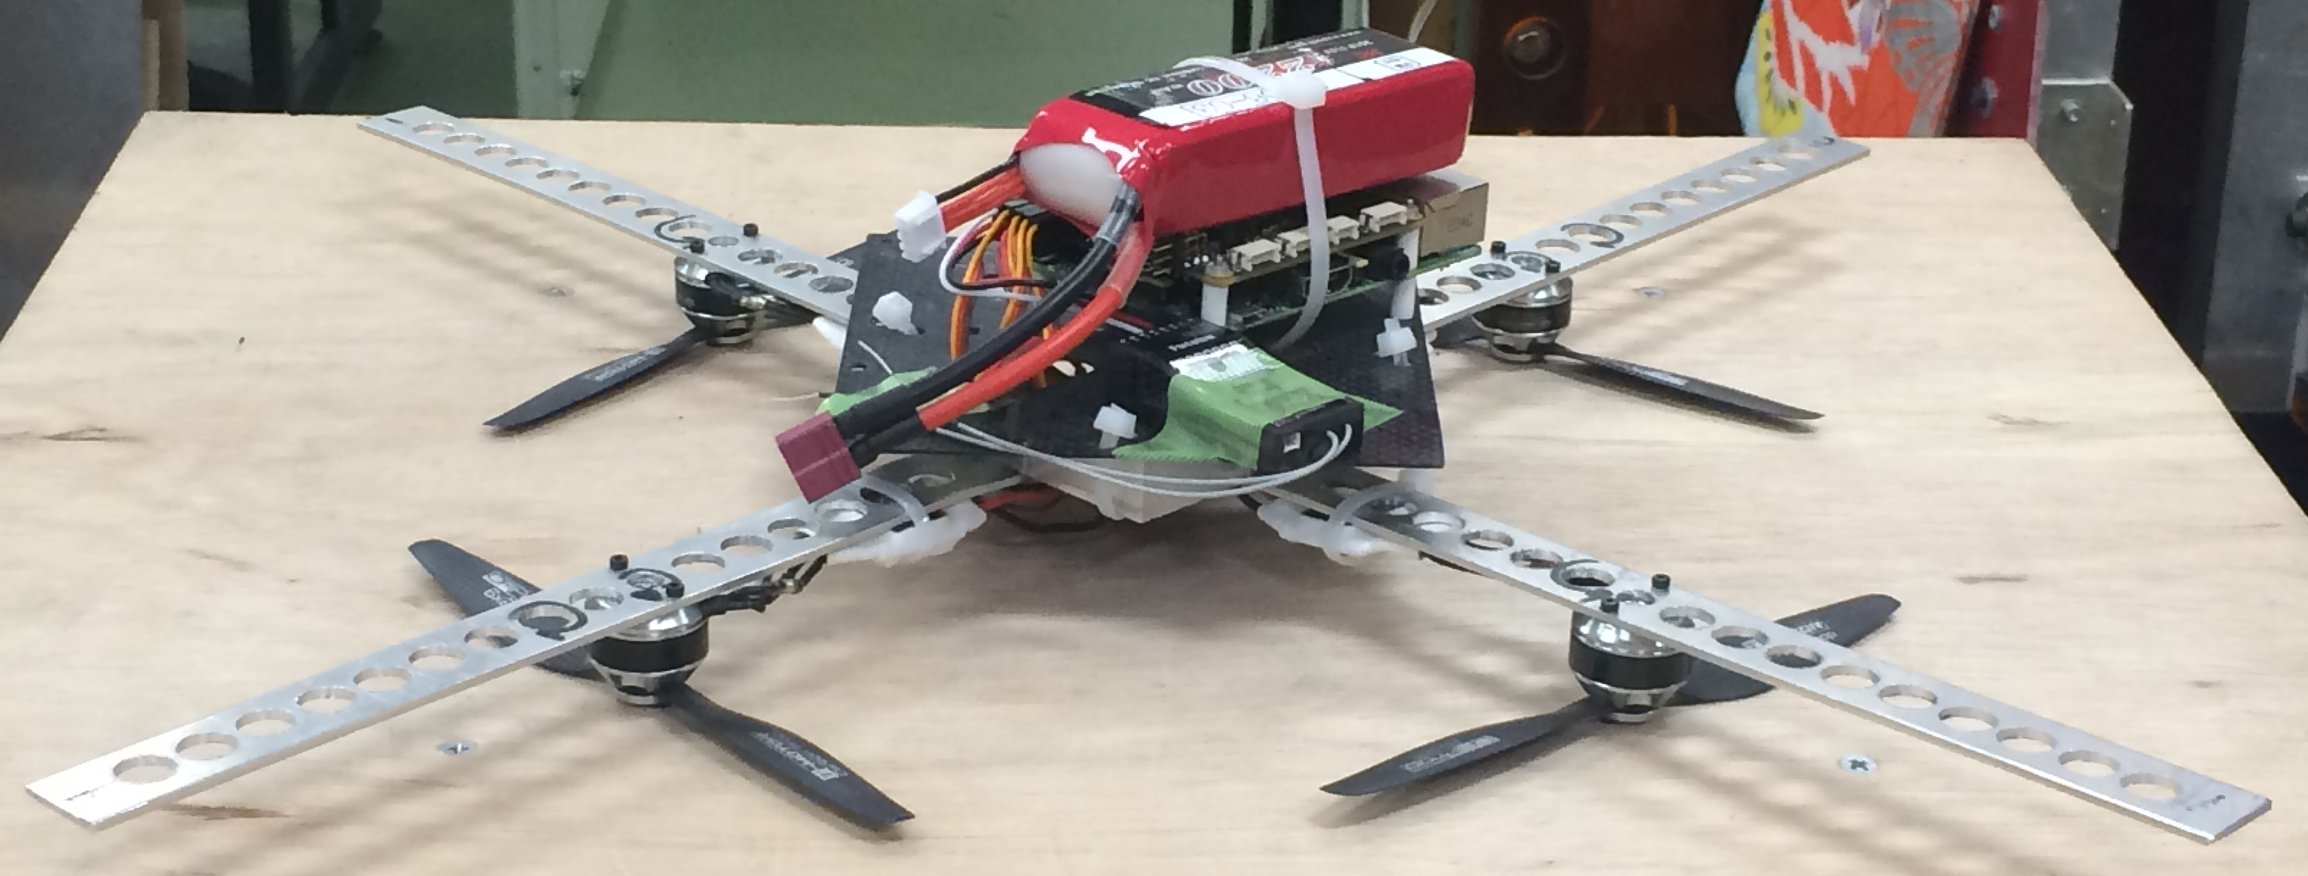
\includegraphics[width=70mm]{image/drone/drone-1.jpg}
		\caption{機体1号機}
		\label{fig:drone-1}
	\end{center}
\end{figure}

\subsubsection{2号機}
アームの強度改善のためアームの断面をコの字型にし,2本のアームが機体中央で交差する形状になっている.
RaspberryPi,バッテリーの固定にはABS樹脂板で専用の取付板を製作し,これらをアームの上下に取り付けている.
製作した2号機を図\ref{fig:drone-2}に示す.
この機体は軽量で製作費も安く非常に良かったが,落下時にアームが曲がってしまった.
このことから塑性変形するアルミをアームに使用するのは難しいと考えた.

\begin{figure}[htbp]
	\begin{center}
		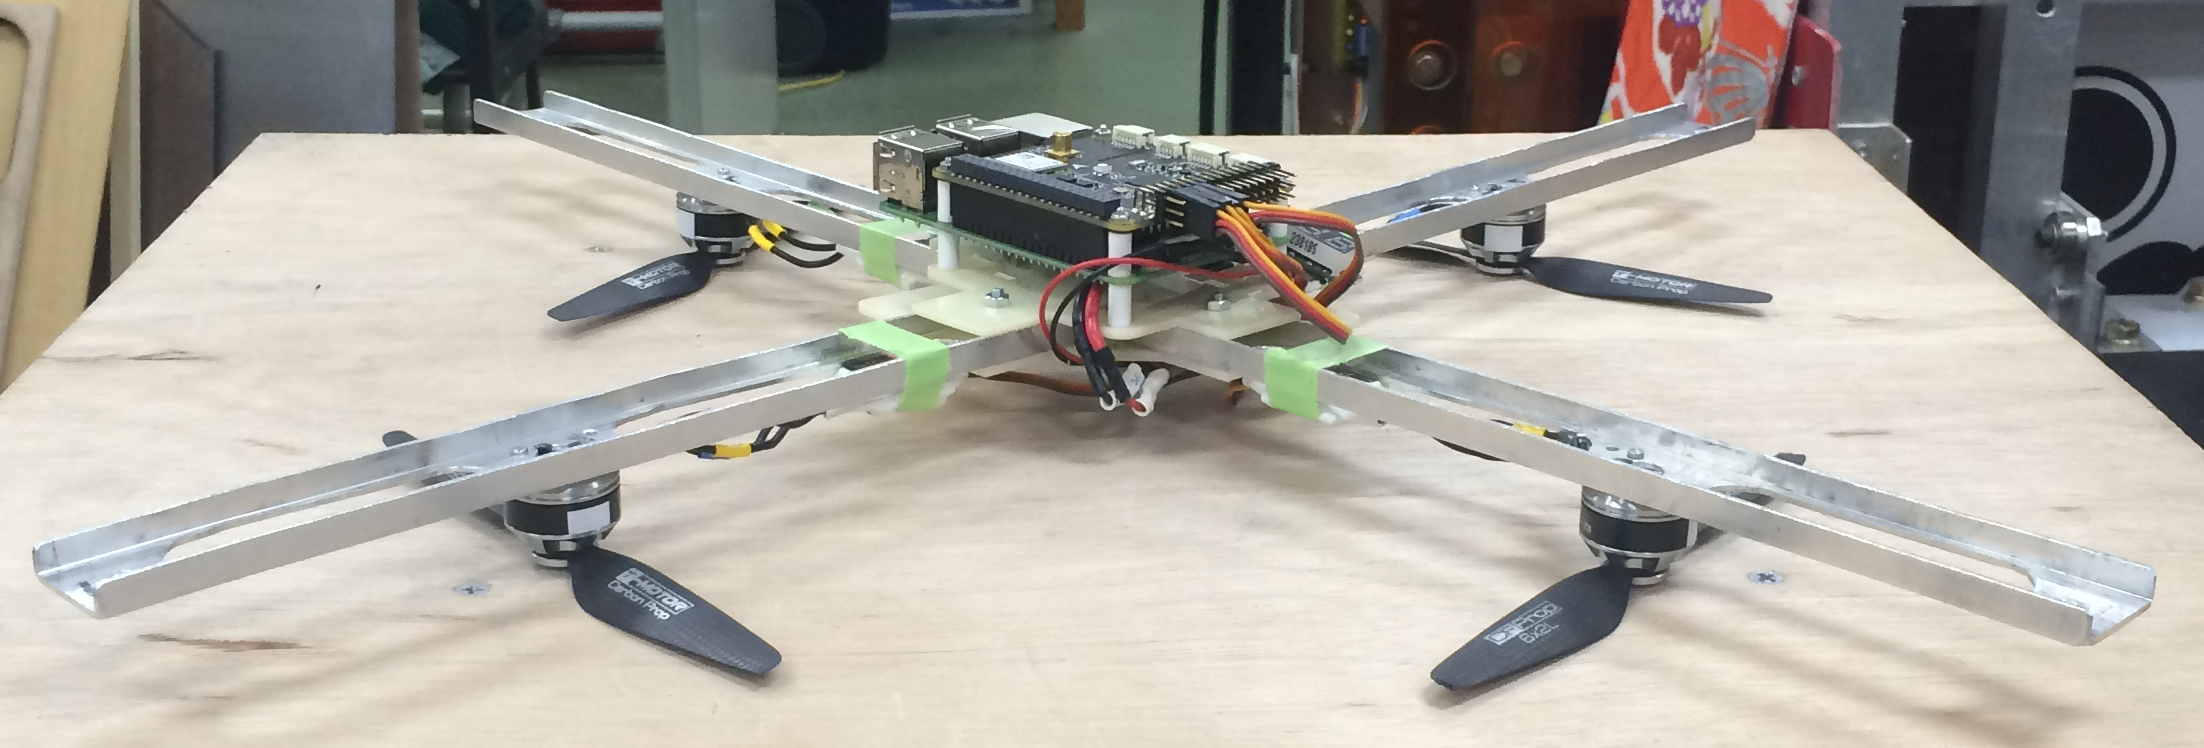
\includegraphics[width=70mm]{image/drone/drone-2.jpg}
		\caption{機体2号機}
		\label{fig:drone-2}
	\end{center}
\end{figure}

\subsubsection{3号機}
アームを塑性変形し難いものにするため,アームに直径12mmのCFRP(炭素繊維強化プラスチック)のパイプを2本ずつ使用している.
このアームをMCナイロンのブロックに穴を開けて半分に切断したもので上下から挟み固定している.
製作した3号機を図\ref{fig:drone-3-1}に示す.
この機体では2号機に比べアームの強度は向上したものの,重量が80g増加してしまった.
また,CFRPのパイプが高価であることやCFRPの加工が容易でないこと,パイプが固定し難いことが問題となった.

\begin{figure}[htbp]
	\begin{center}
		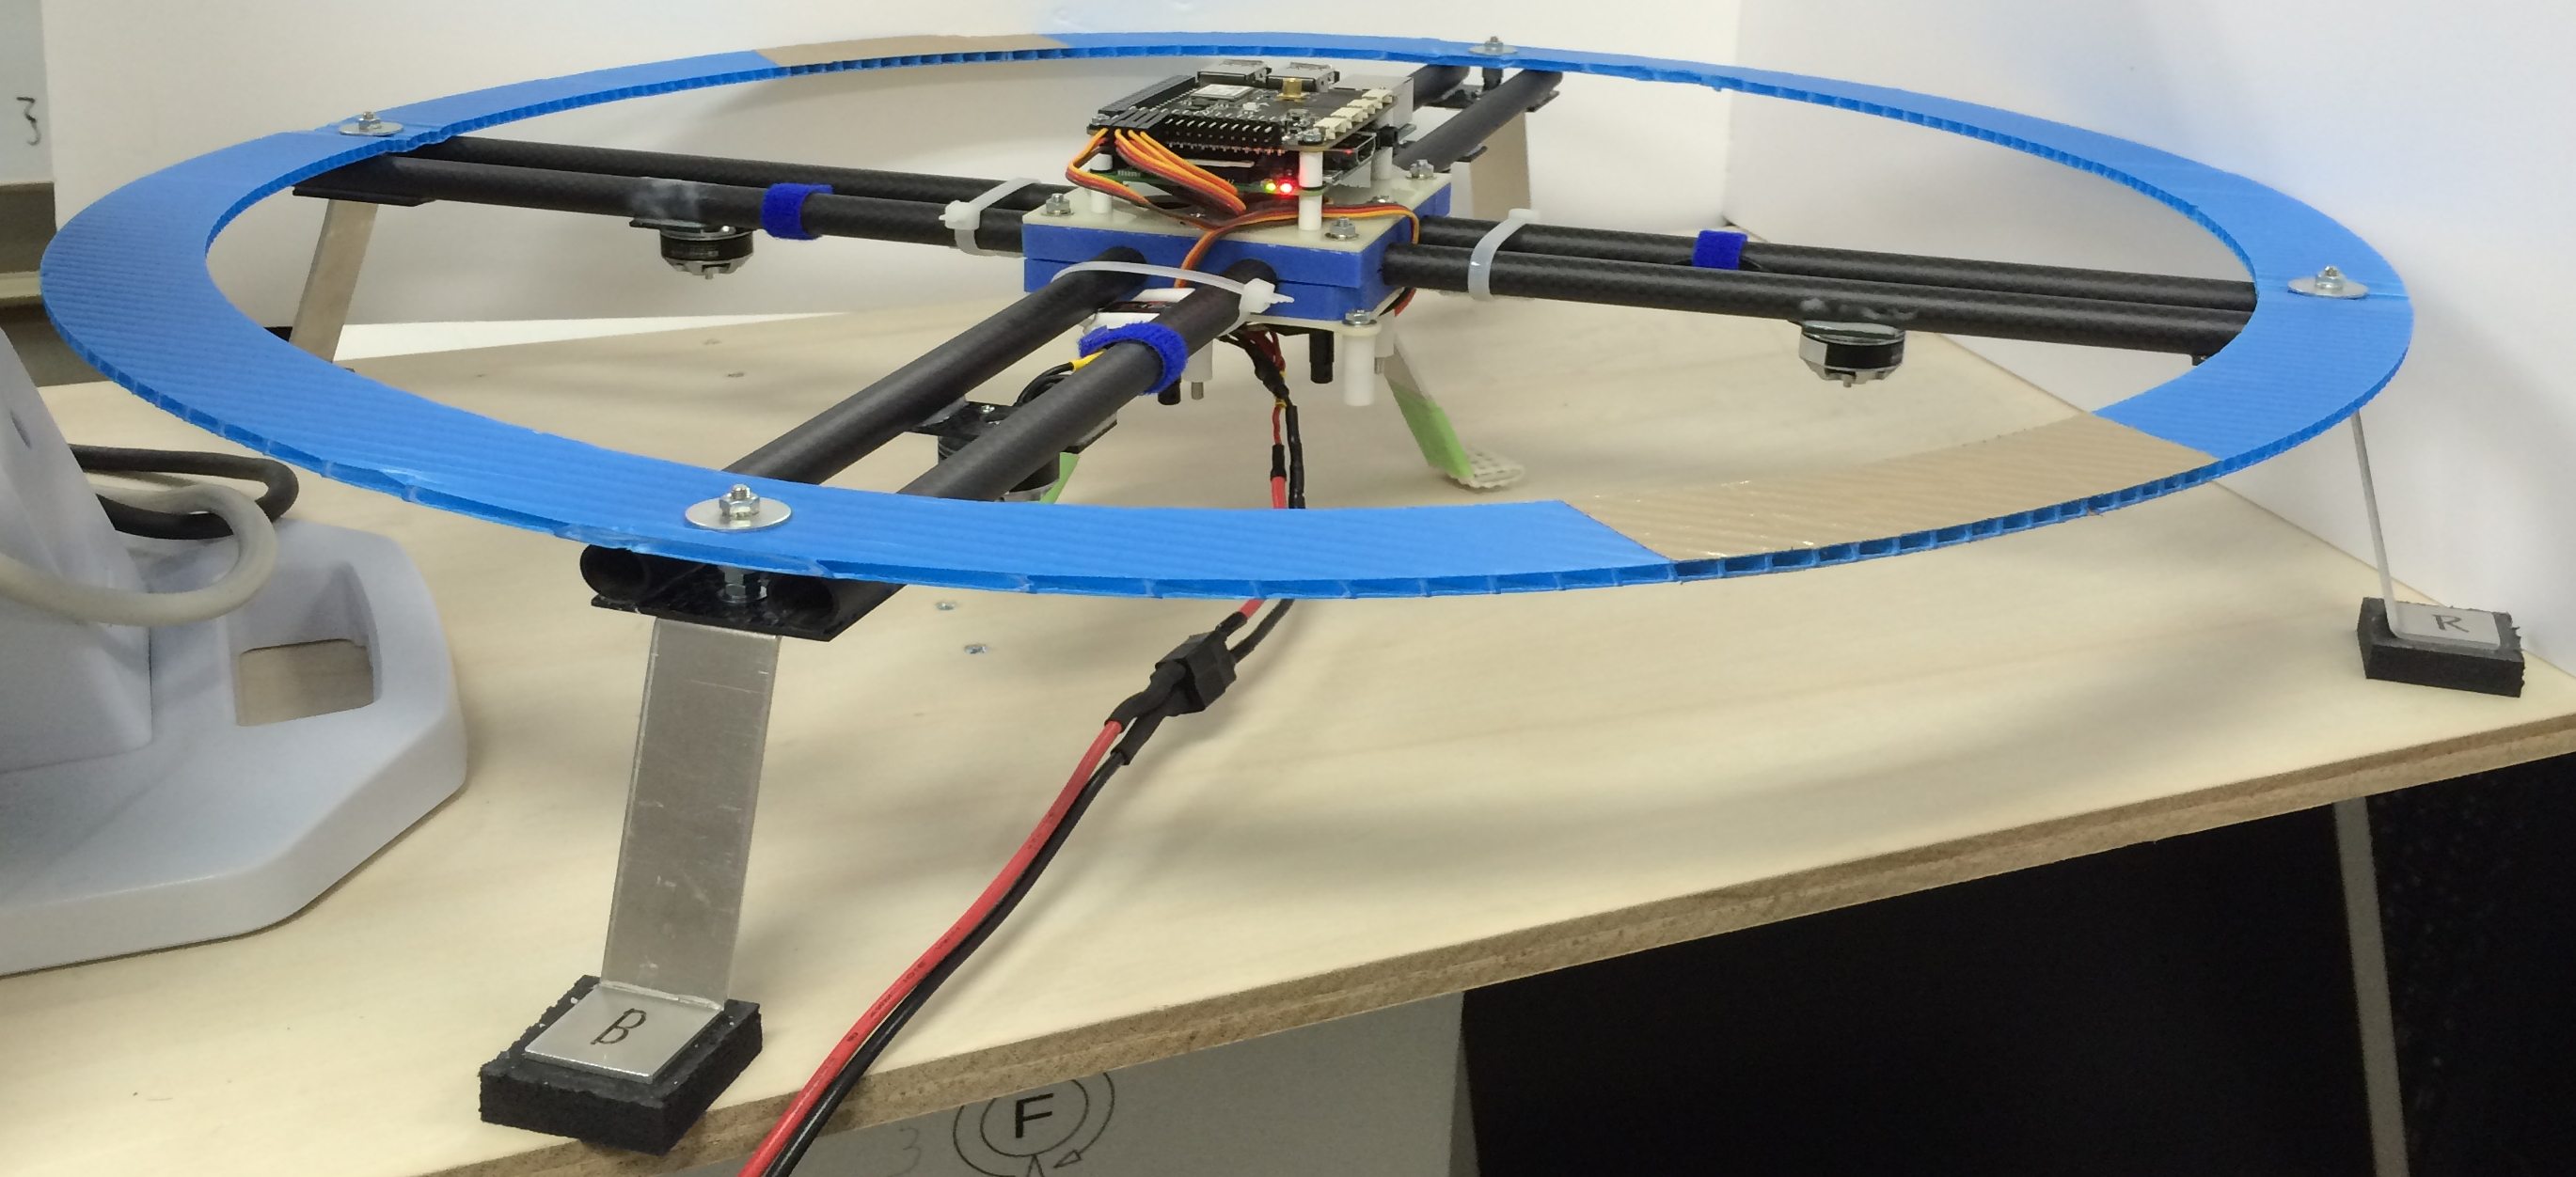
\includegraphics[width=70mm]{image/drone/drone-3-1.jpg}
		\caption{機体3号機}
		\label{fig:drone-3-1}
	\end{center}
\end{figure}

\subsubsection{3号機改}
3号機を軽量化するため,アームの固定に使用するパーツに変更を加えた.
厚さ3mmの木の板のパーツと15mm×15mm,厚さ1.5mmのアルミ角管を用いてアームの固定を行う.
また,木材を使用していためあるアルミ製アームのように塑性変形が発生せず,より安価である.
さらにこの改善により70gの軽量化を達成した.
製作した3号機改を図\ref{fig:drone-3-2}に示す.

\begin{figure}[htbp]
	\begin{center}
		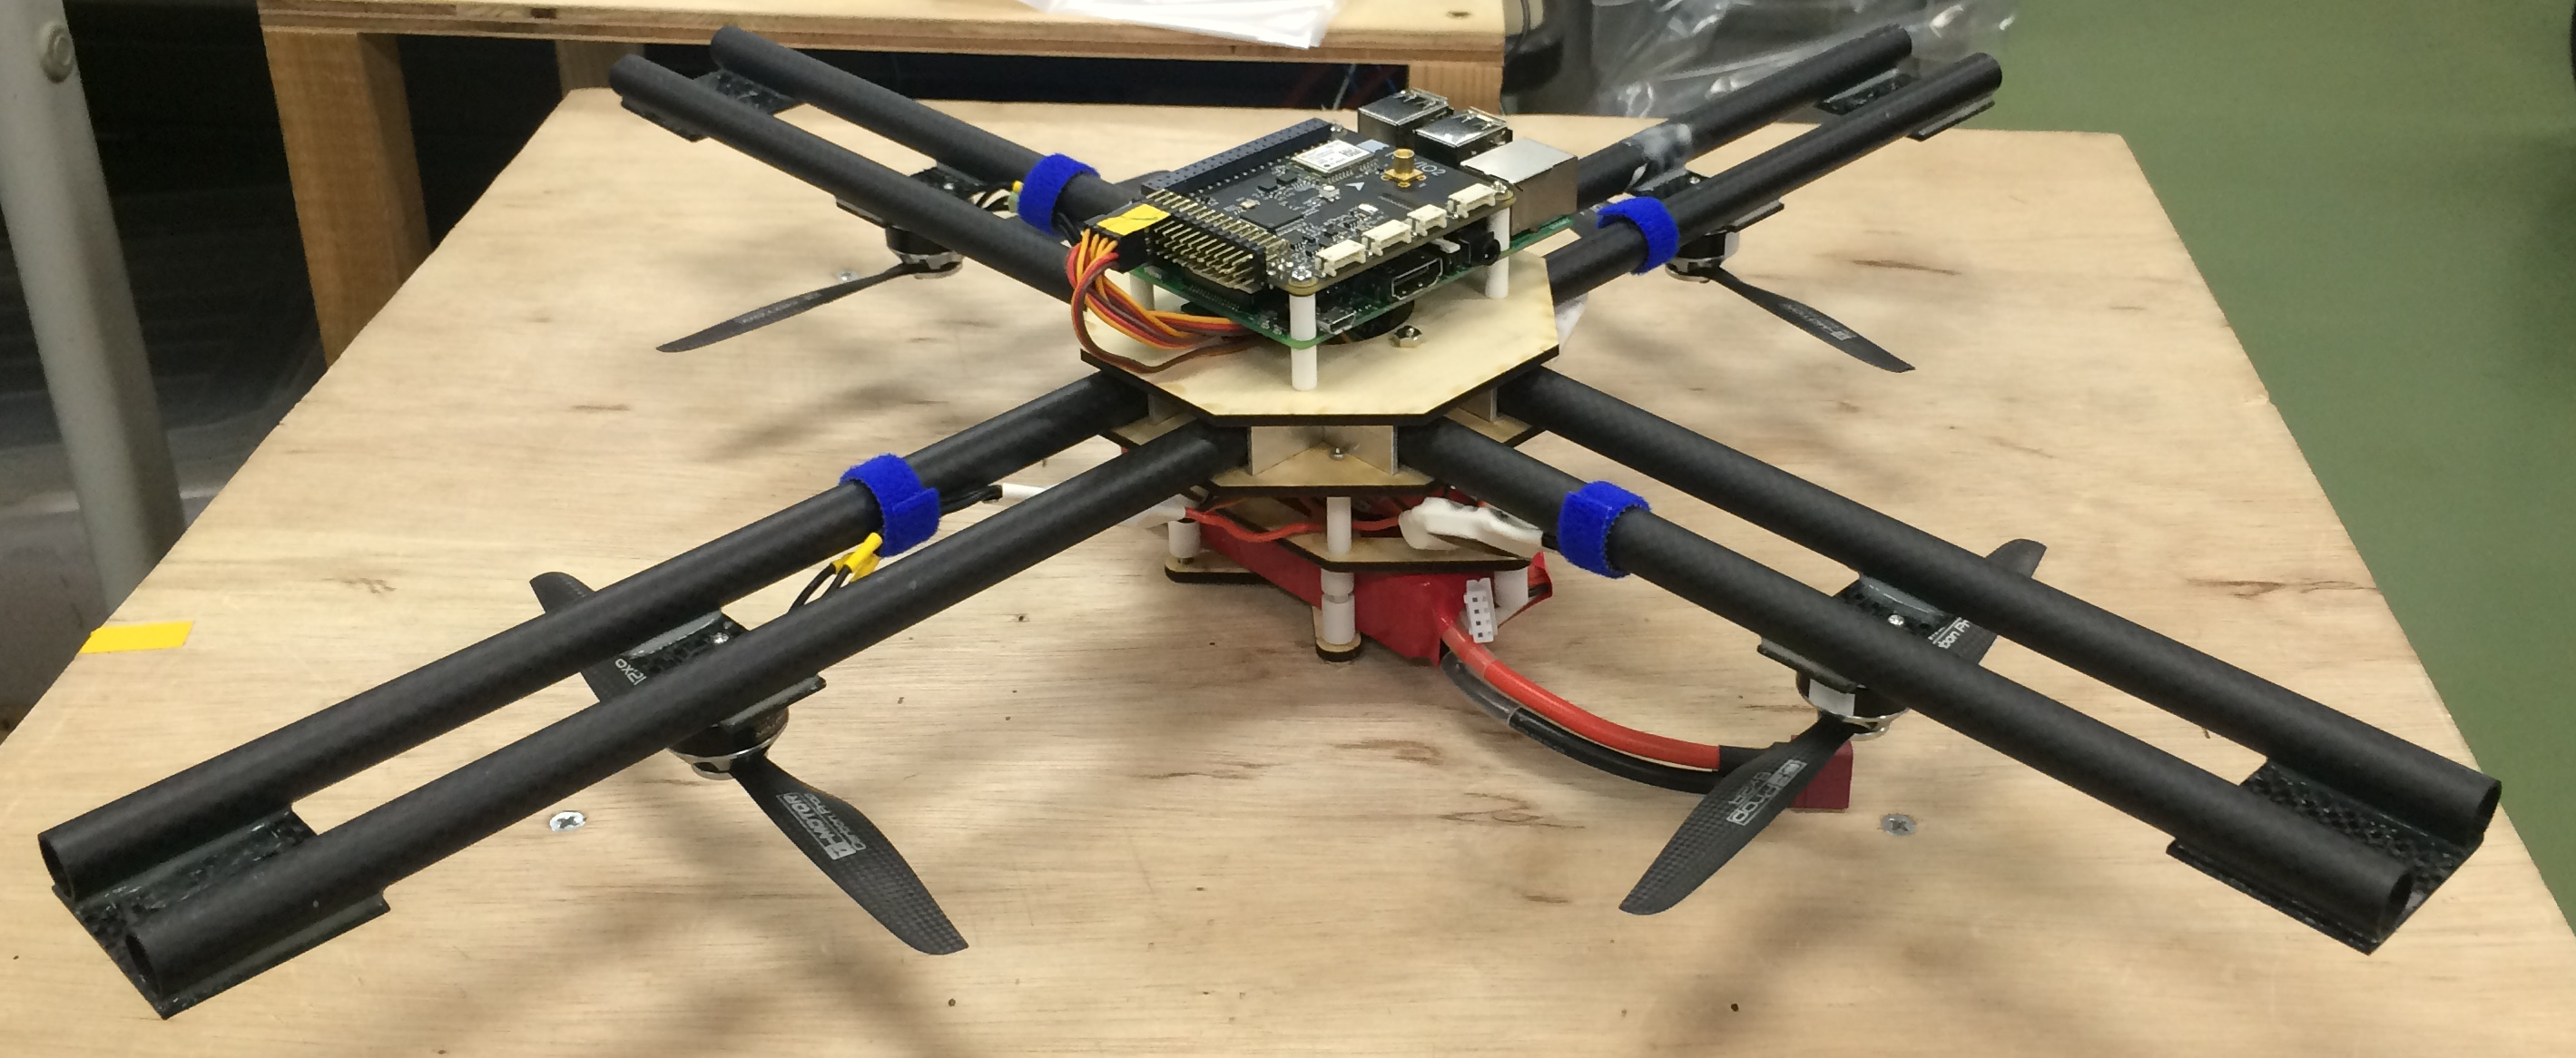
\includegraphics[width=70mm]{image/drone/drone-3-2.jpg}
		\caption{機体3号機改}
		\label{fig:drone-3-2}
	\end{center}
\end{figure}

\subsection{球体}

\subsubsection{1号機}
1号機では厚さ5mmのスチレンボードからパーツを切り出し,接合部は接着剤で固定している.
製作した1号機を図\ref{fig:sphere-1}に示す.
この球体は落下時の衝撃で接合部周辺のスチレンと紙が剥離し壊れてしまった.

\begin{figure}[htbp]
	\begin{center}
		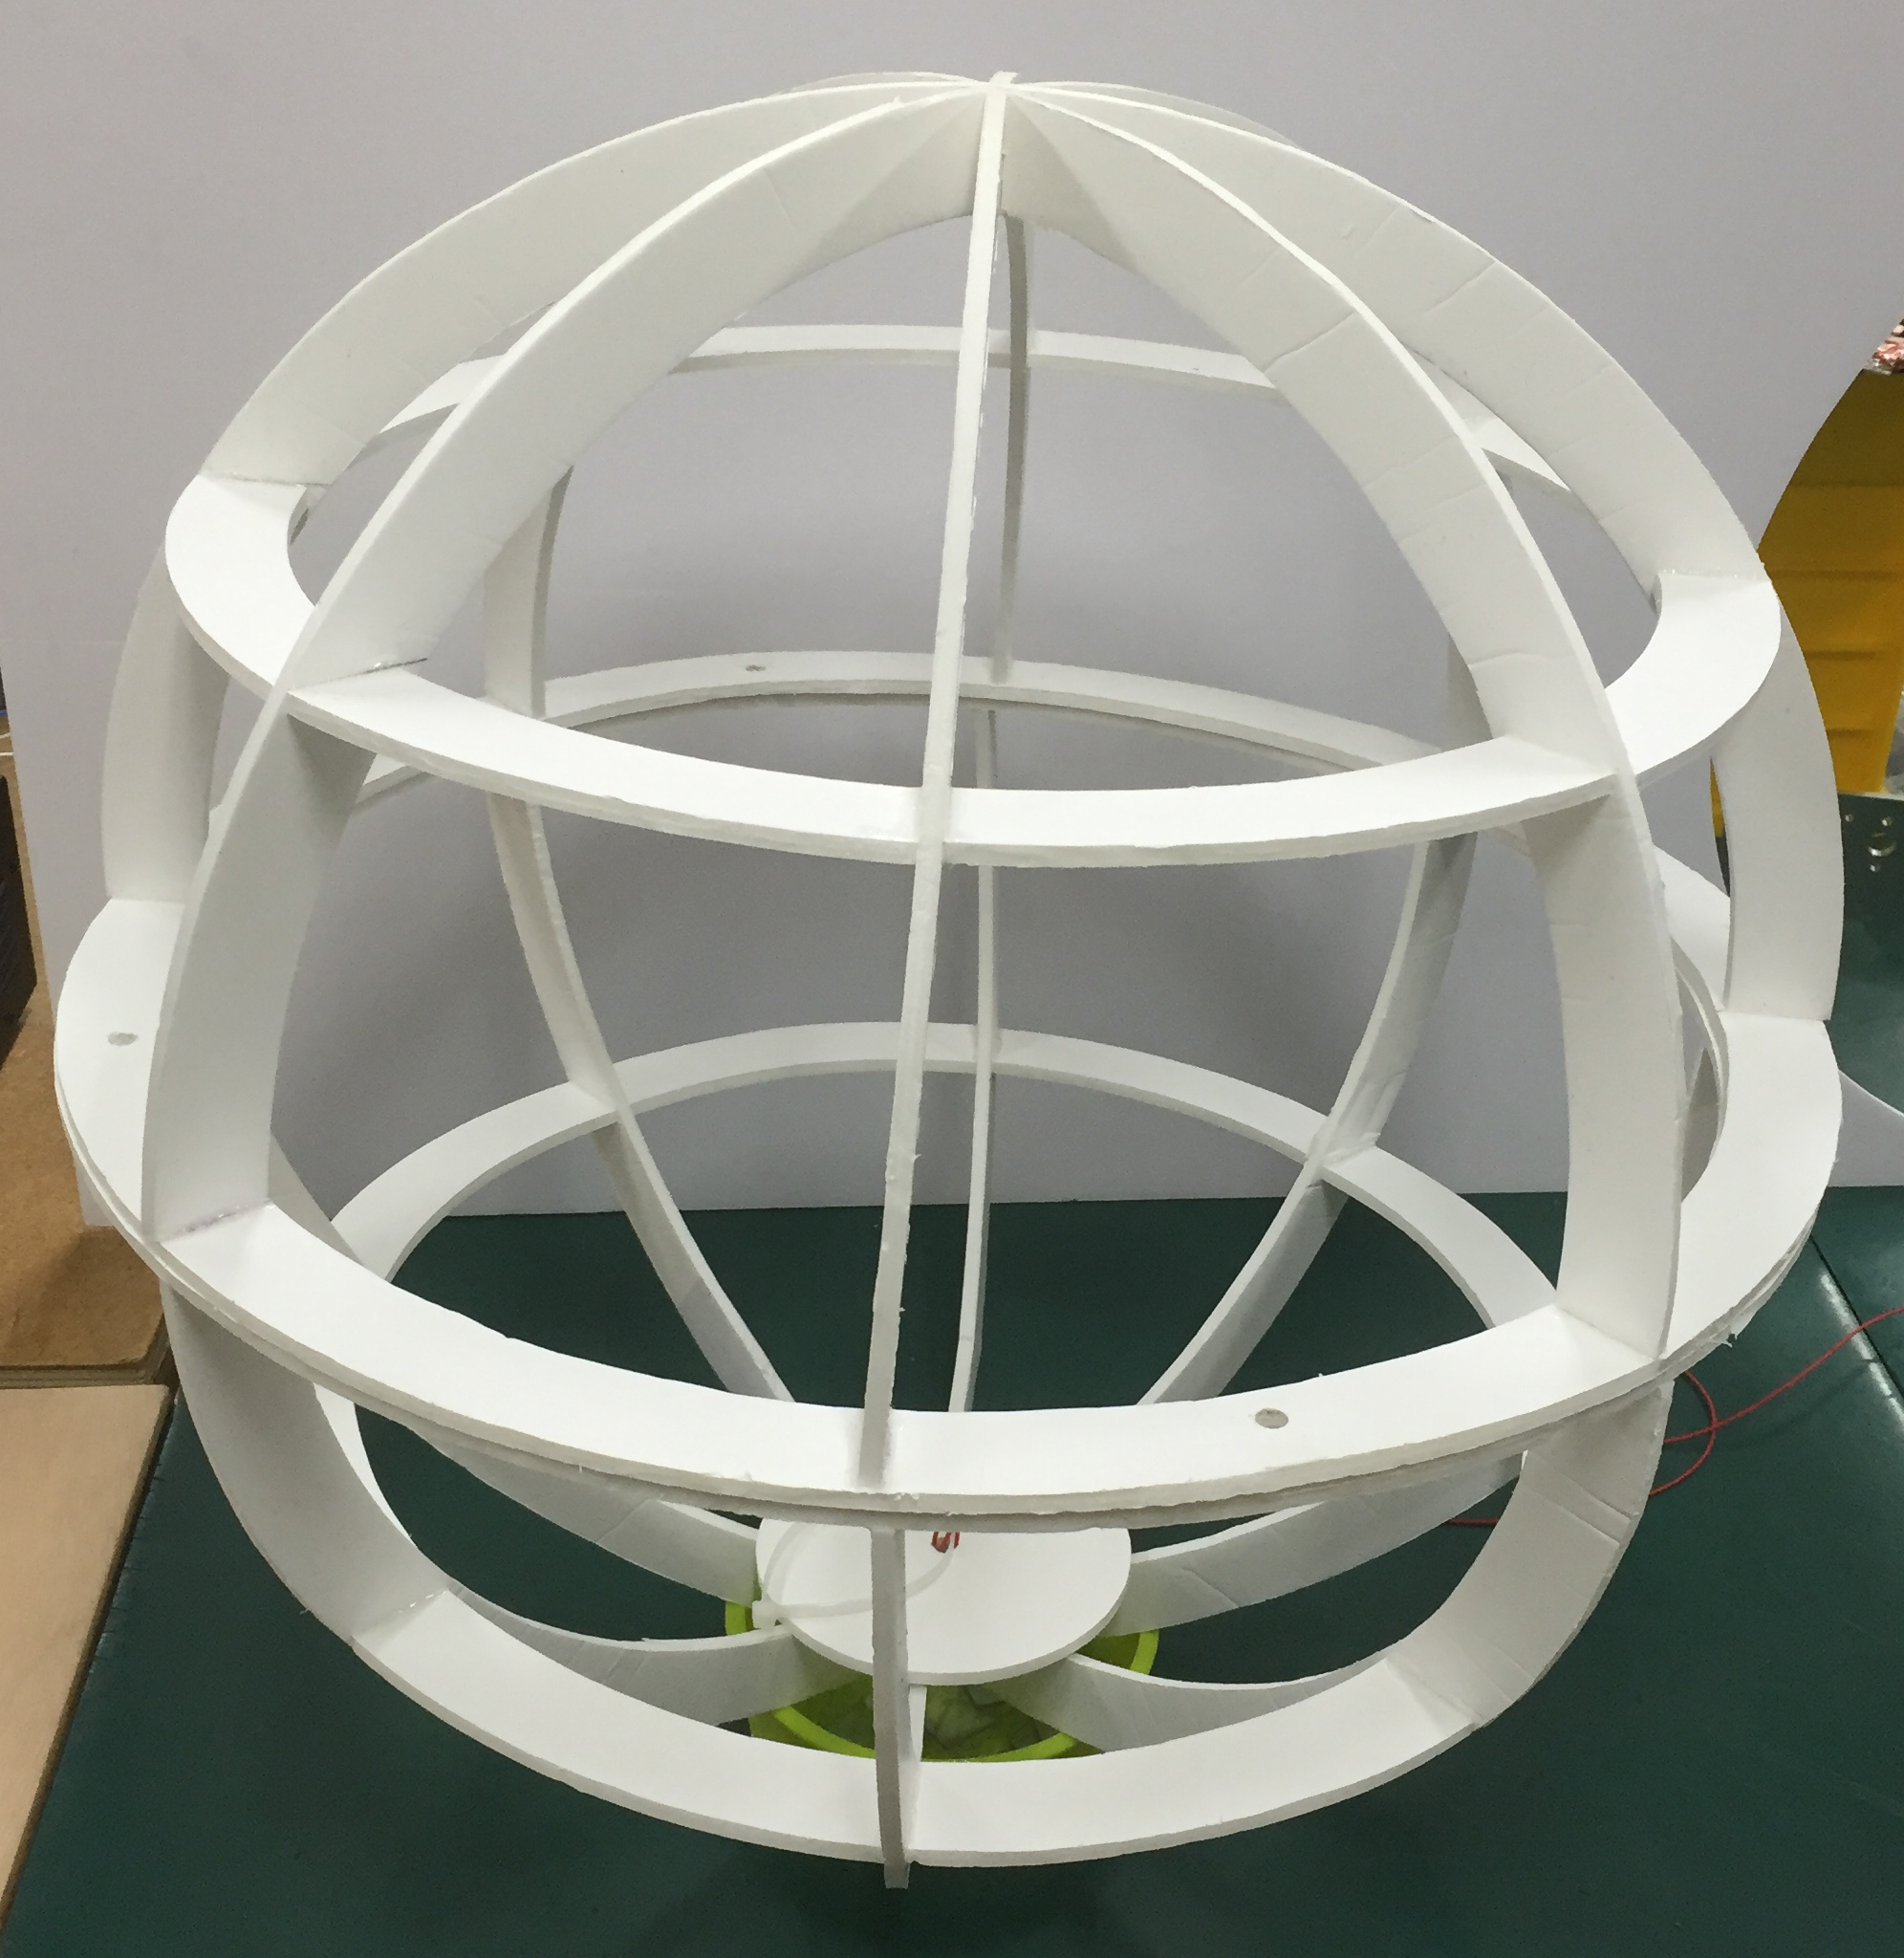
\includegraphics[width=60mm]{image/sphere/sphere-1.jpg}
		\caption{球体1号機}
		\label{fig:sphere-1}
	\end{center}
\end{figure}

\subsubsection{2号機}
接合部でのスチレンと紙の剥離が起こらないように接合部に図\ref{fig:kigumi}のような木組み構造を取り入れた.
これによりスチレンと紙の剥離は起こらなくなった.
製作した2号機を図\ref{fig:sphere-2}に示す.

\begin{figure}[htbp]
	\begin{center}
		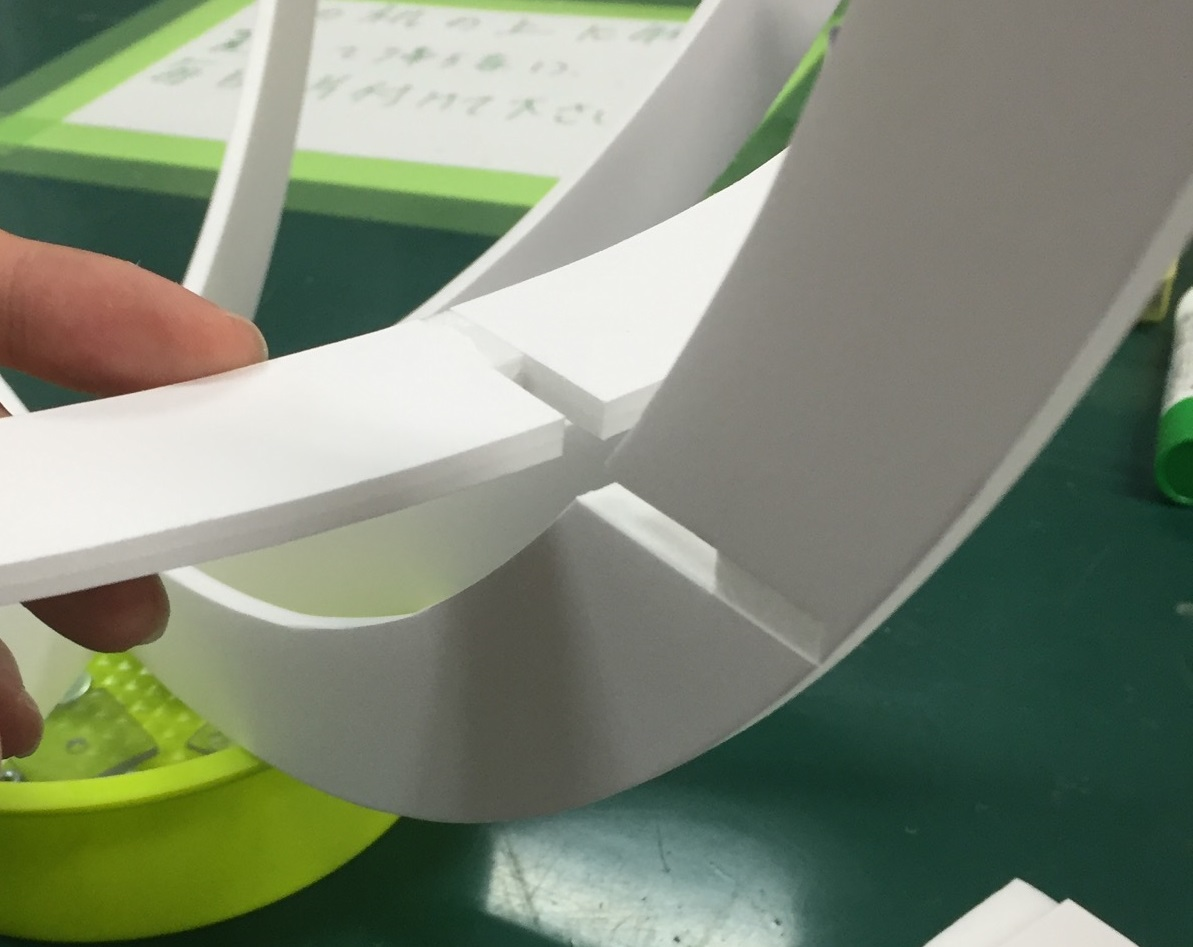
\includegraphics[width=60mm]{image/sphere/kigumi.jpg}
		\caption{木組み部分}
		\label{fig:kigumi}
	\end{center}
\end{figure}

\begin{figure}[htbp]
	\begin{center}
		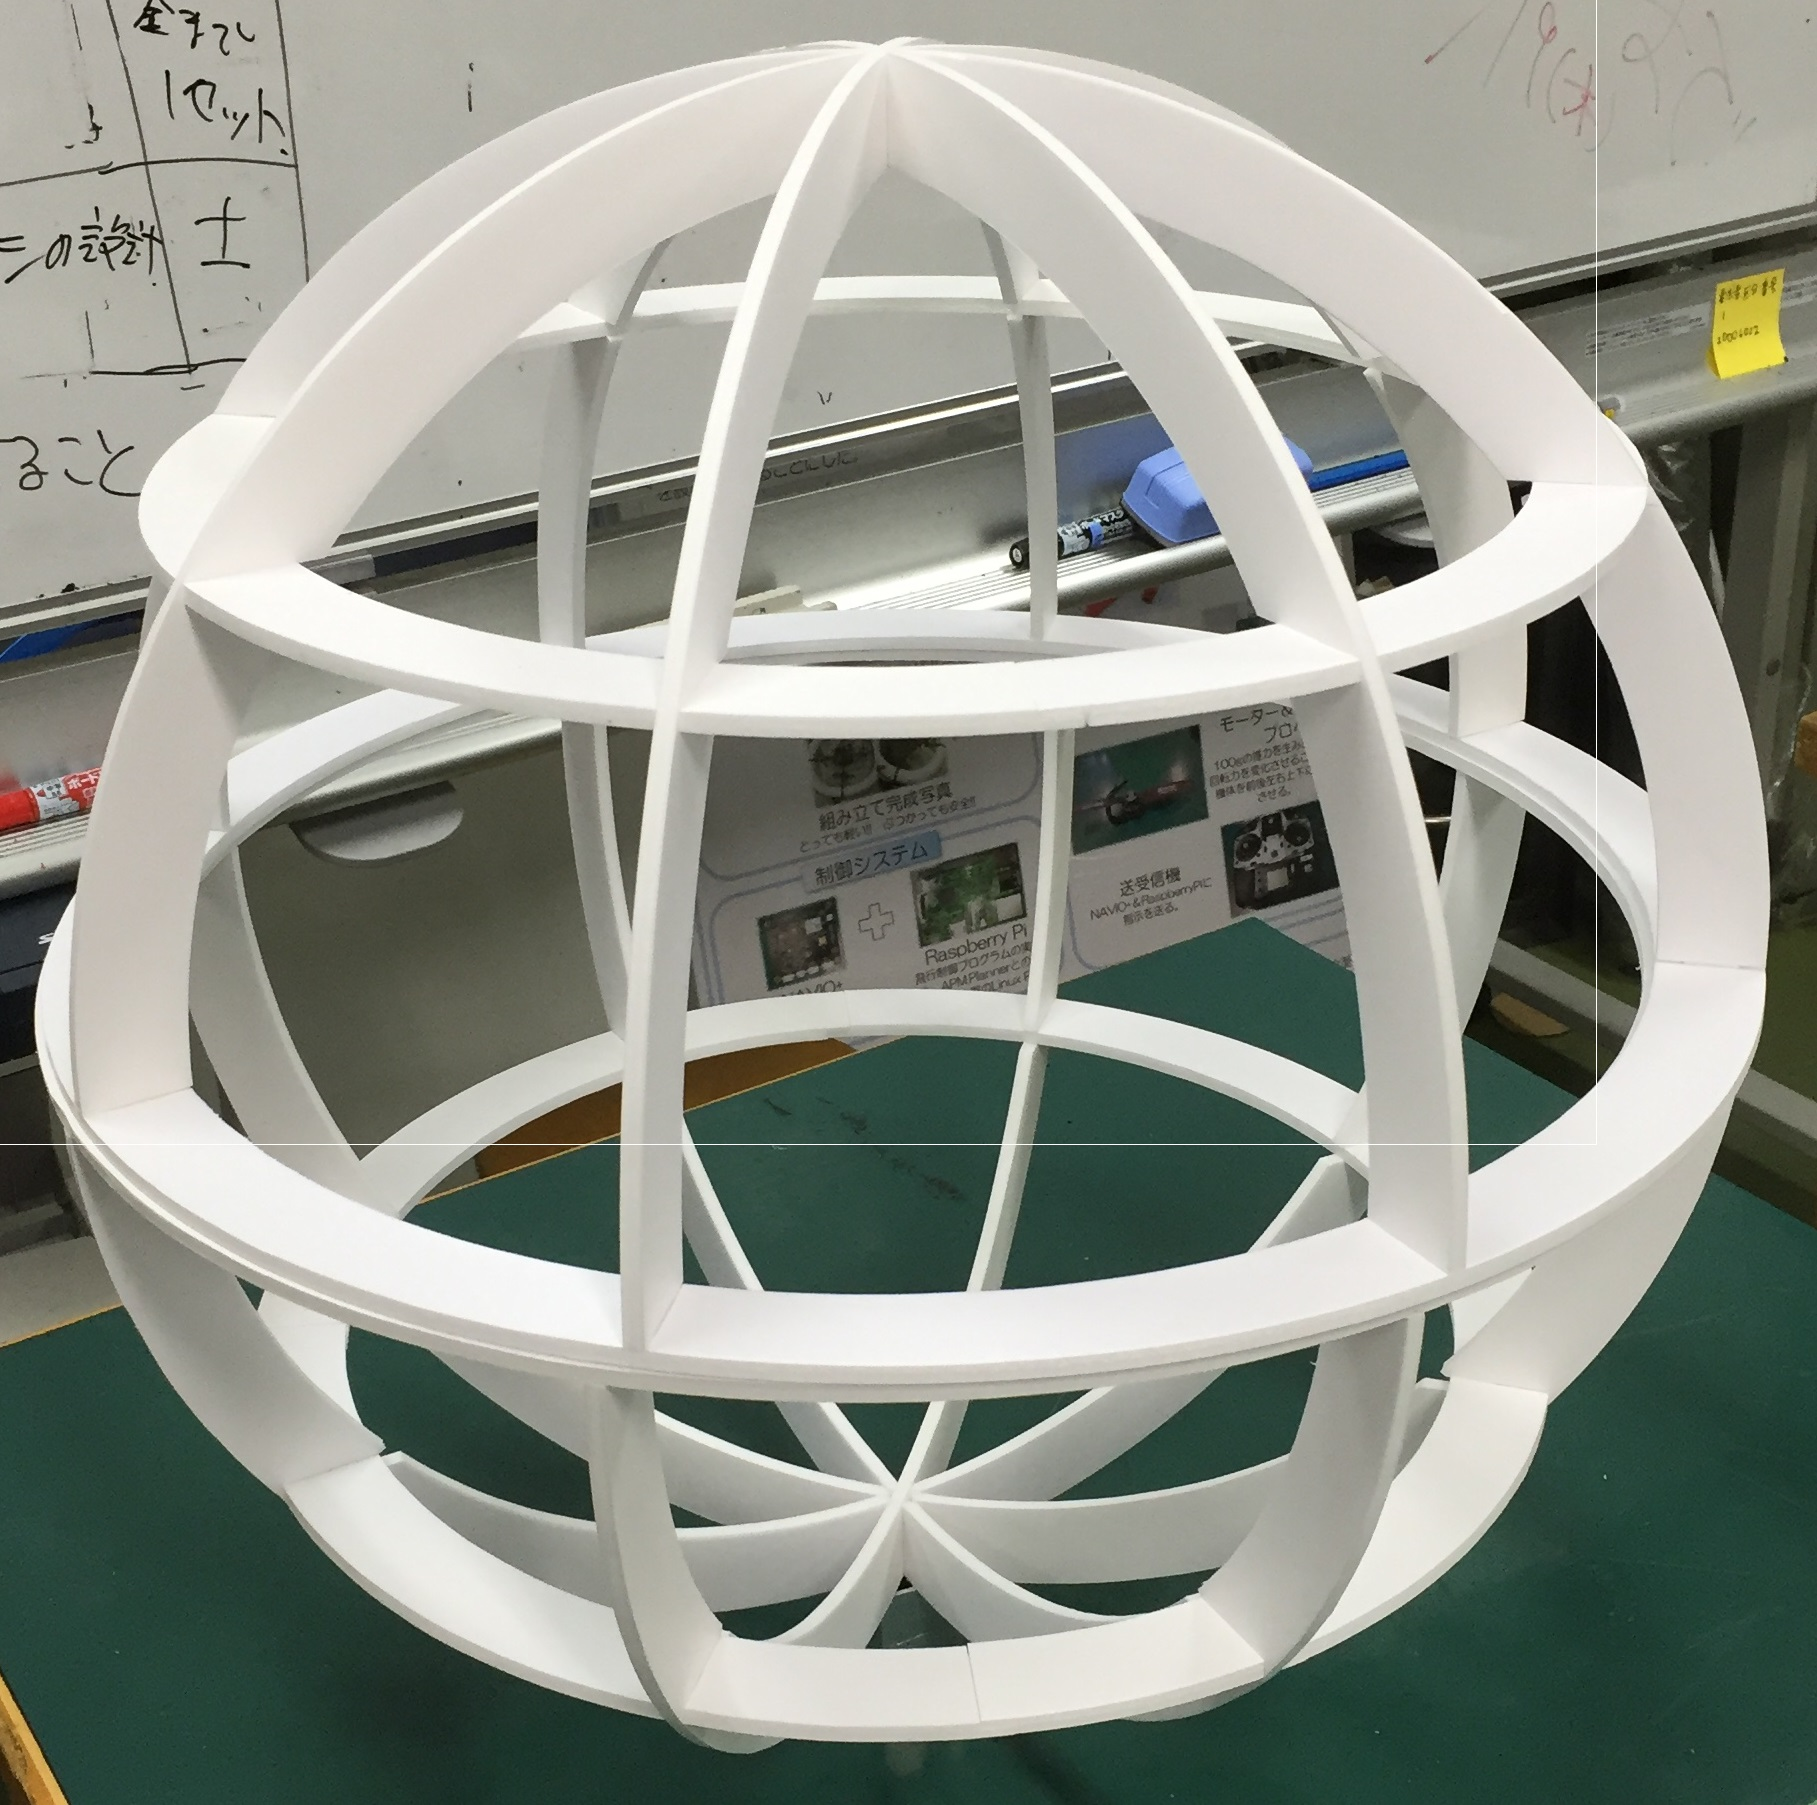
\includegraphics[width=60mm]{image/sphere/sphere-2.jpg}
		\caption{球体2号機}
		\label{fig:sphere-2}
	\end{center}
\end{figure}

\subsubsection{3号機}
1号機,2号機では手作業でパーツを切り出していたため製作に時間がかかっていた.
そのためパーツの切り出しにかかる時間を短縮するため,パーツの切り出しをすべてレーザー加工機で行うことにした.
これにより製作時間の大幅な短縮に加え,加工精度の向上ができた.
製作した3号機を図\ref{fig:sphere-3}に示す.

\begin{figure}[htbp]
	\begin{center}
		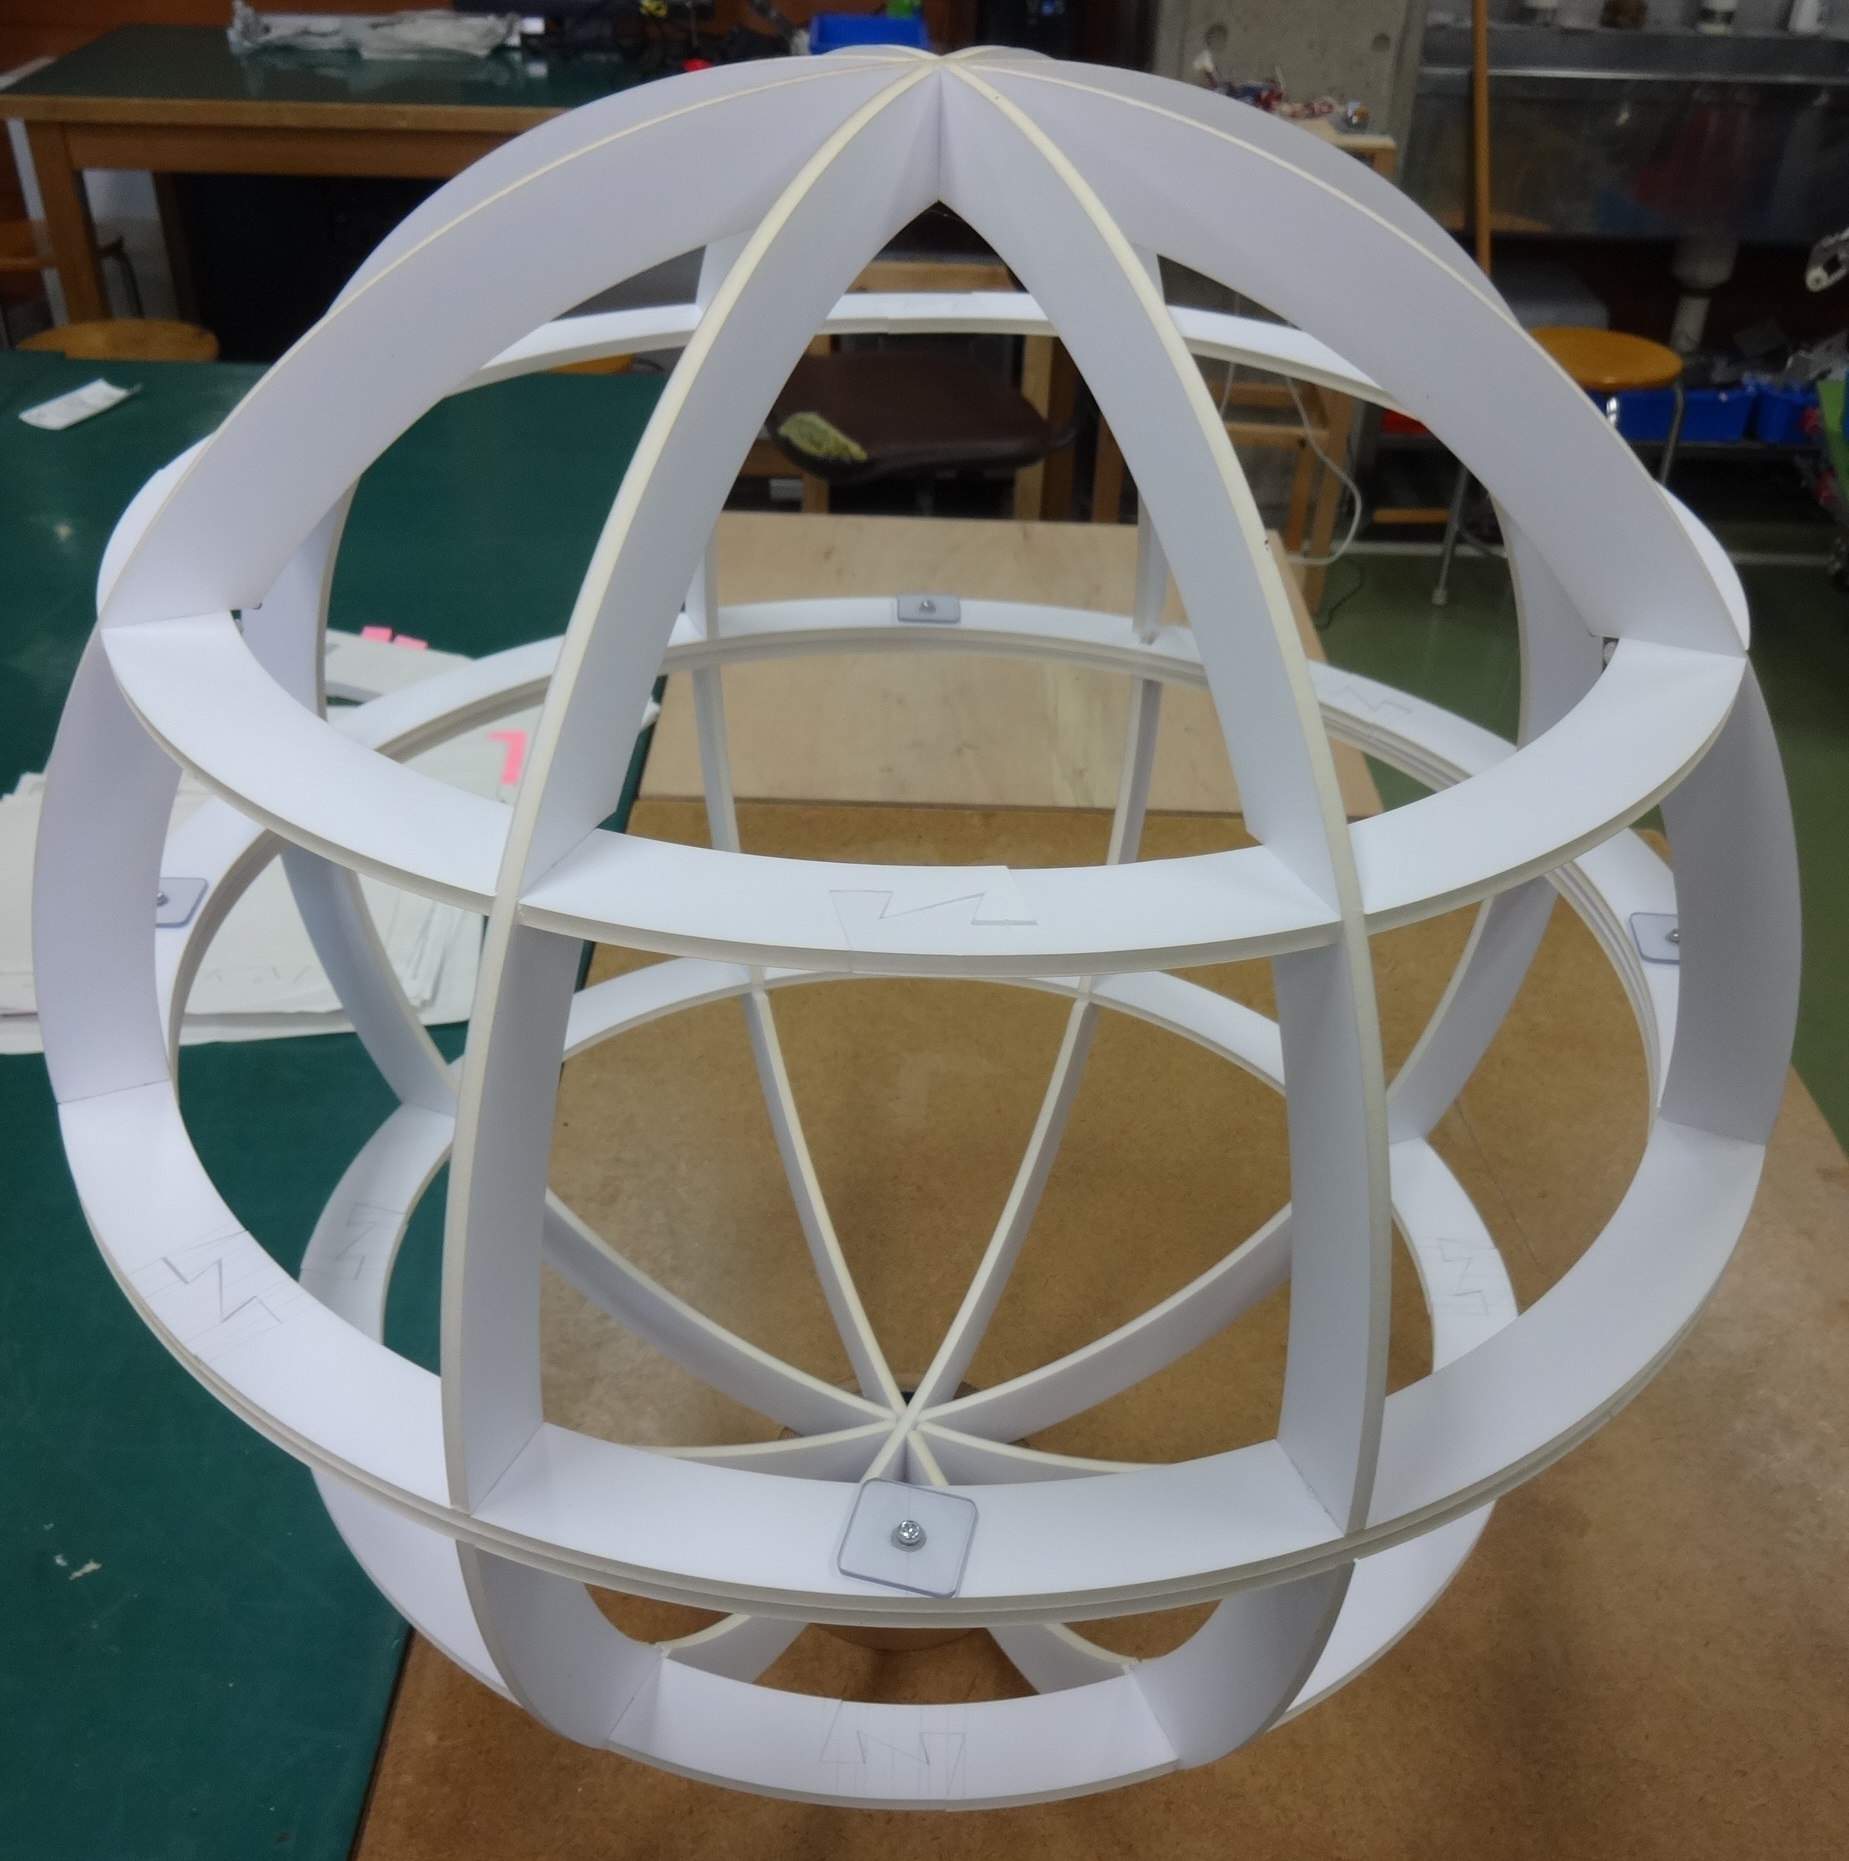
\includegraphics[width=60mm]{image/sphere/sphere-3.jpg}
		\caption{球体3号機}
		\label{fig:sphere-3}
	\end{center}
\end{figure}

\section{理想的な機体,球体の仕様}
第3節からわかるように,機体では強度,重量が大きな問題となった.
3号機改で木の板からレーザー加工機でパーツの切り出しを行ったことから,機体全体を木の板から切り出して製作する手法が考えられた.
木の板は安価であり衝撃吸収にも優れていることからマルチコプターのアームに適していると考えた.
現在の機体は図\ref{fig:CD-data}のようなデータをレーザー加工機に入力することで,図\ref{fig:cut}のようにパーツを簡単に切り出すことができる.

\begin{figure}[htbp]
	\begin{center}
		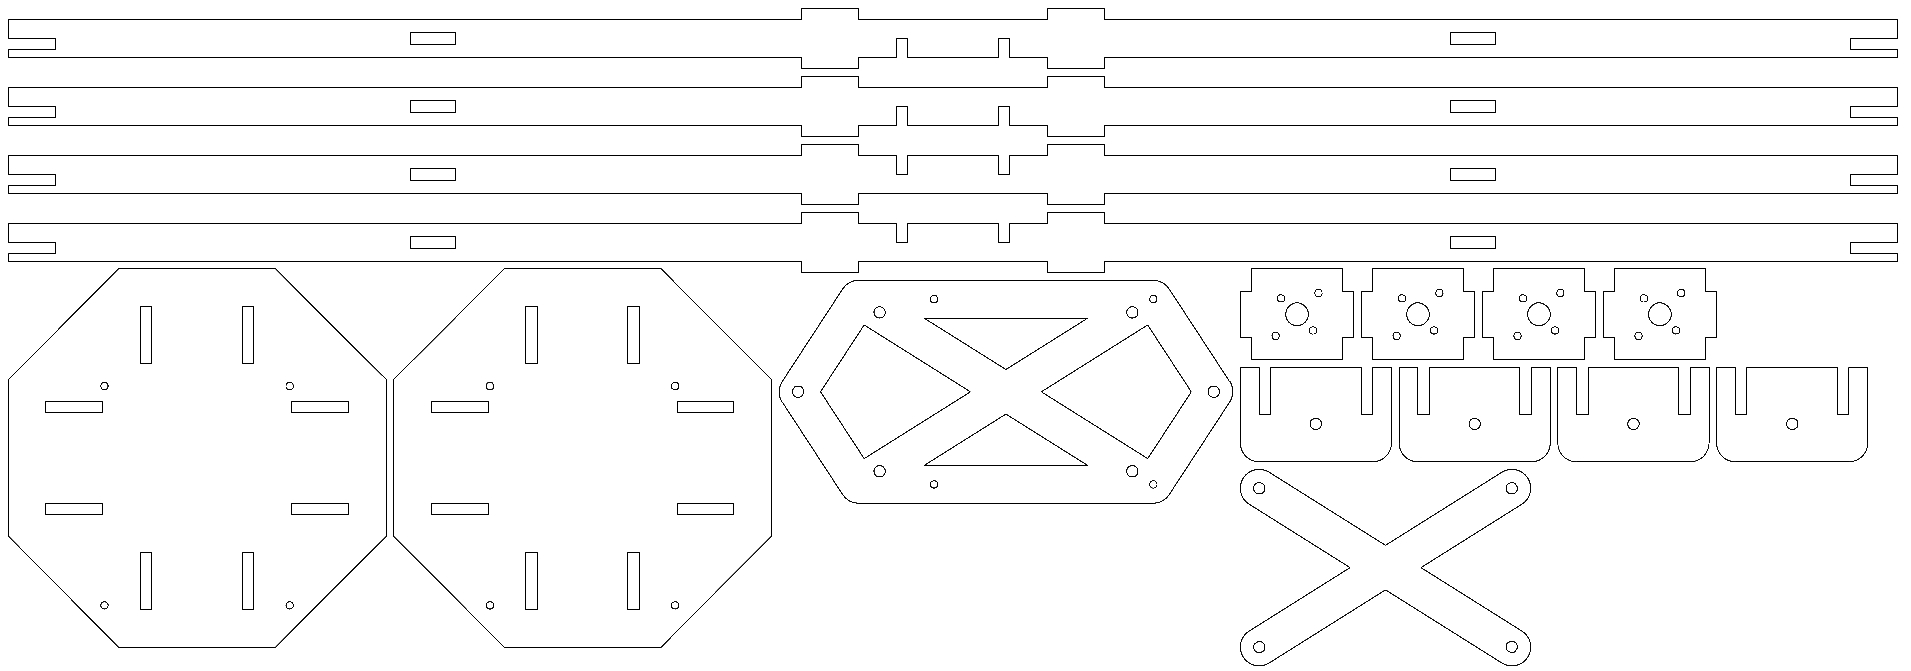
\includegraphics[width=80mm]{image/drone/CD-data.jpg}
		\caption{機体パーツの切り出し用データ}
		\label{fig:CD-data}
	\end{center}
\end{figure}

\begin{figure}[htbp]
	\begin{center}
		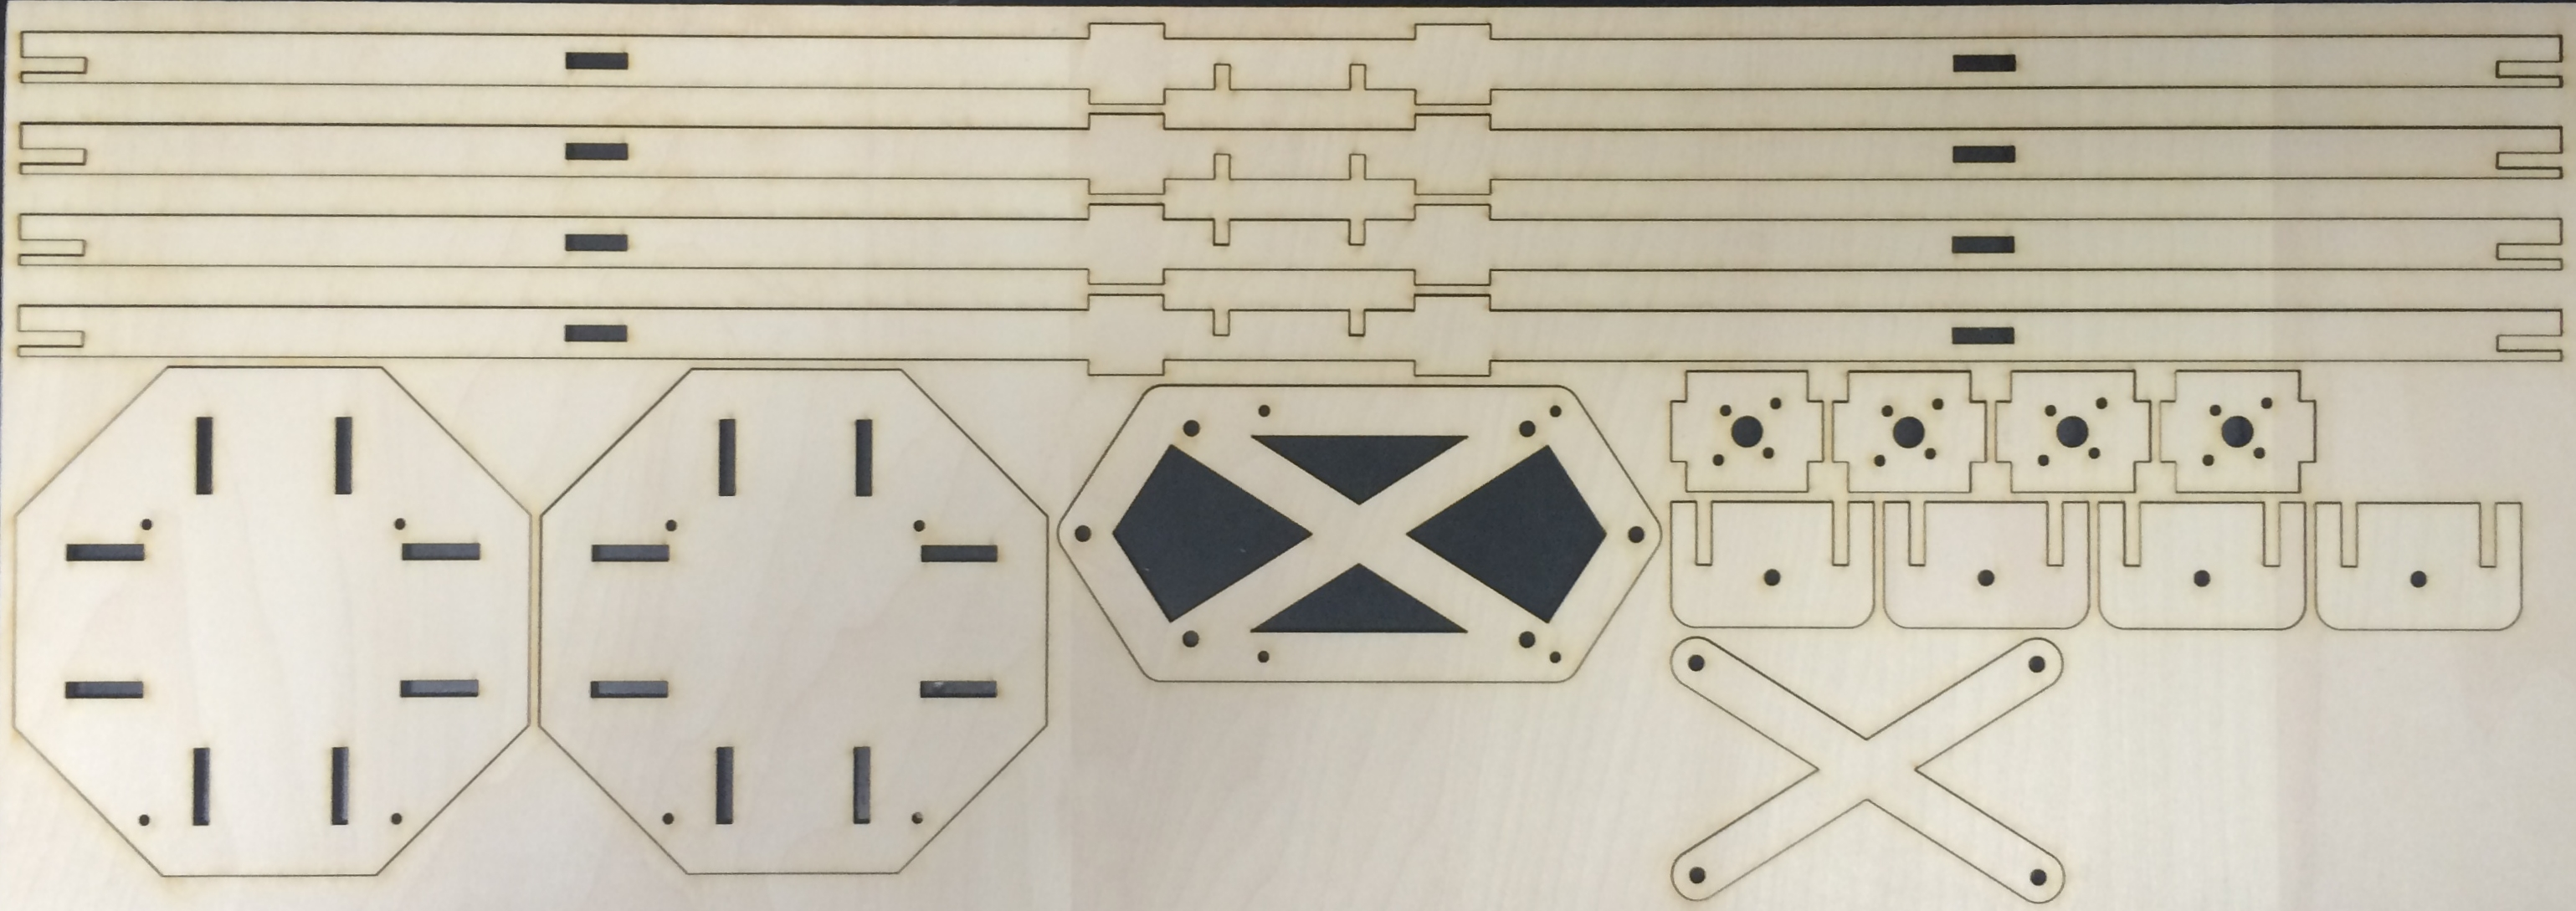
\includegraphics[width=80mm]{image/drone/cut.jpg}
		\caption{実際に切り出した機体パーツ}
		\label{fig:cut}
	\end{center}
\end{figure}

球体の1から3号機は全て飛行試験中に幾度も墜落する内に破損してしまった.
そこで材料の改良が必要であると考え,耐衝撃性に優れるポリプロピレン製のプラスチックダンボールを使用することとなった.

現在のマルチコプターの総重量は717gである.
後述の推力特性の確認実験から4つのモータ,プロペラにより発生する推力は最大で1099gであることがわかっている.
機体の姿勢制御を行うことを考慮すると,総重量を最大推力の8割以下にしたいと考える. %何割にしましょうか


\chapter{ソフトウェア}

\section{目標}
一般的なマルチコプター同様,コントローラ操作により上昇・下降,前後左右の移動,右・左旋回を行えるようにする.

\section{概要}
航空機力学の座標系\cite{config}に準じ,図\ref{fig:config}のように座標系を設定している.
角変位は右ねじの法則に従いx軸回りをロール,y軸回りをピッチ,z軸回りをヨーとする.
コンピュータにRaspberryPi3 ModelB,センサモジュールにNavio2,コントローラにDUALSHOCK3を使用する.
Bluetooth通信によりRaspberryPiとDUALSHOCK3を接続し,スティック操作により操作を行う.

\begin{figure}[htbp]
	\begin{center}
		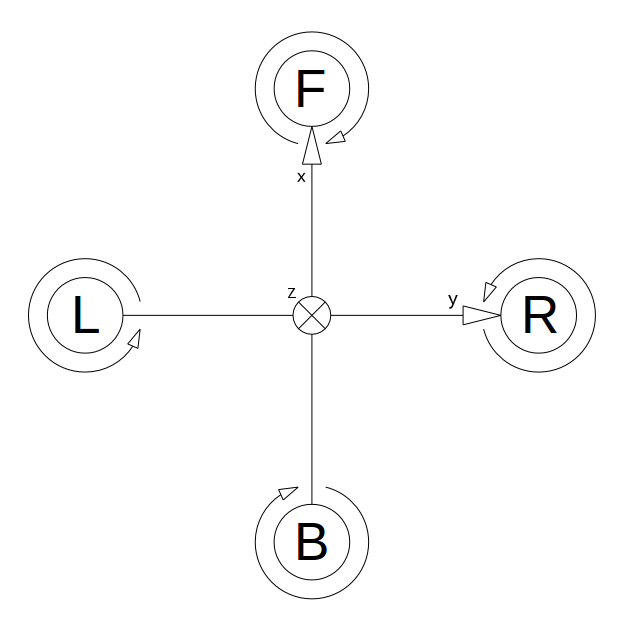
\includegraphics[width=55mm]{image/config.png}
		\caption{座標系の設定}
		\label{fig:config}
	\end{center}
\end{figure}

\section{開発環境}
開発に使用した機材,ソフトウェアなどを表\ref{table:dev}に示す.

\begin{table}[htbp]
	\begin{center}
		\caption{開発環境}
		\begin{tabular}{|l|l|} \hline
			 & windows7 \\
			パソコン & ubuntu 16.04 LTS \\
			 & ubuntu 14.04 LTS \\ \hline
			RaspberryPi OS & emlid-raspbian-20160718 \\ \hline
			コンパイラ & g++ \\ \hline
			 & Scilab \\
			数値計算ソフト & Microsoft Excel \\
			 & gnuplot \\ \hline
		\end{tabular}
		\label{table:dev}
	\end{center}
\end{table}

\section{コントローラ}
前述の通りコントローラはDUALSHOCK3をBluetooth通信で接続し使用する.
ペアリングにはsixpair,SixaxisジョイスティックマネージャーにはQtSixAを使用している.
ペアリング,Bluetooth通信についての詳細は付録に記載する.
右スティックの前後方向をスロットル,左右方向をヨー方向制御,左スティックで前後左右移動する.
また,スタートボタンで一時停止/再開,一時停止中にセレクトボタンでプログラムが終了する.
Navio2のLEDがプログラムが動作していない時は緑に,プログラム動作中は赤に,一時停止中は青に点灯する.

\section{プログラムの流れ}
はじめにセンサやコントローラなどの設定を行い,静止状態でジャイロセンサの校正を行う.
続いて無限ループに入りコントローラ,センサ情報の取得,各種計算,モータ制御の順に繰り返す.
また,この無限ループ中でコントローラの入力値やセンサ情報,モータへの出力値などをテキストファイルに書き出している.

\section{PID制御}
当初はPID制御によりモータ制御を行っていた.

PIDとは比例(Proportional),積分(Integral),微分(Differential)の頭文字をとったものである.
PID制御は目標値と現在の値の差に比例,積分,微分をそれぞれ行い,それらに補正値ゲインを掛けて足し合わせることで必要な制御量を求める制御方式である.\cite{pid}

\section{PID制御での飛行試験}
製作した機体1号機と球体1号機を組み合わせ,天井から紐で吊るして飛行試験を行った.
この状態ではコントローラ操作に対し問題なく動作した.

機体2号機と球体2号機を組み合わせ,地面に張ったネットの上で飛行させた.
ここで墜落し球体が破損したため,一時的に足を取り付けた.

機体3号機に現在の球体を取り付け,地面に置いた状態からの飛行を試みた.
しかし,足を取り付けた状態では姿勢が安定していたのに対し,球体カバーを取り付けた状態では姿勢が不安定なため傾きが発散し離陸することができなかった.
球体カバーを取り付けた状態で離陸を試みた際の角速度をグラフ化したものを図\ref{fig:test-1}に示す.

\begin{figure}[htbp]
	\begin{center}
		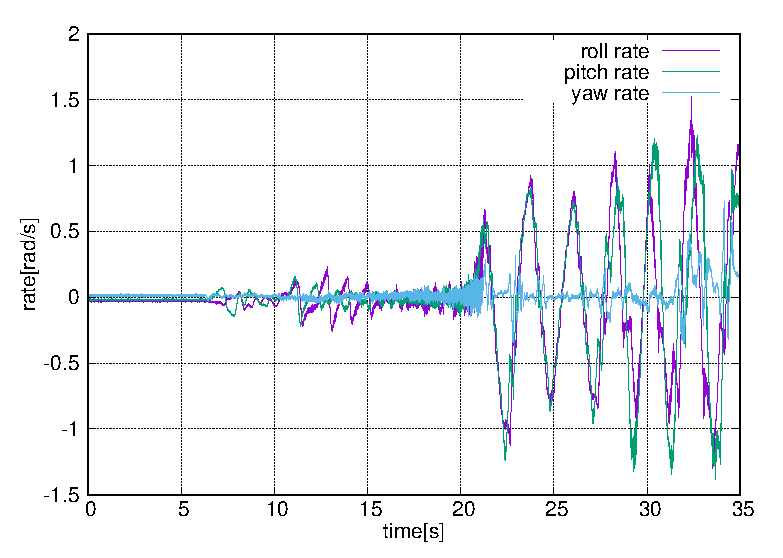
\includegraphics[width=75mm]{image/test-1.eps}
		\caption{離陸時の角速度}
		\label{fig:test-1}
	\end{center}
\end{figure}

以上からPID制御だけでは球体カバーを取り付けた状態での離陸は困難であることが判明した.
制御系の設計を見直し,最適レギュレータを設計することにした.

\section{最適レギュレータ設計までの流れ}

\subsection{運動方程式}
運動方程式には航空機の運動方程式を利用する.
前提条件として,左右対称,前後非対称,上下非対称,傾きが微小であることなどがある.
この方程式をルンゲ・クッタ法を用いて解く.
ルンゲ・クッタ法とは微分方程式を数値的に解く方法である.以下に実際に使用するルンゲ・クッタ法で代表的なルンゲ・クッタ法の公式を示す.

\begin{equation}
	x_k+1 = x_k+\frac{1}{6}h(k_1+2k_2+2k_3+k_4)
	\label{eq1}
\end{equation}

\begin{equation}
	k_1 = f(x_k,t_k)
	\label{eq2}
\end{equation}

\begin{equation}
	k_2 = f(x_k+\frac{hk_1}{2},t_k+\frac{h}{2})
	\label{eq3}
\end{equation}

\begin{equation}
	k_3 = f(x_k+\frac{hk_2}{2},t_k+\frac{h}{2})
	\label{eq4}
\end{equation}

\begin{equation}
	k_4 = f(x_k+hk_3,t_k+h)
	\label{eq5}
\end{equation}

この公式の特徴は,独立変数tが, \(t_k\) , \(t_k+2h\) , \(t_k+2h\) , \(t_k+h\) と単調に増加していることである.したがって,変数tに \(t=t_k\) と入れたらt=t+h/2 , t=t+h/2と2回代入文を繰り返してtを増加させれば,手順の終了時には, \(t=t_k+1\) となっている.


未知関数xの値も, \(t_k\) (t= \(t_k\)の値)から始まって

\(k_1\)を求めて \(x_k+\frac{1}{6}hk_1\)             x=x+1/6k


\(k_2\)を求めて \(x_k+\frac{1}{6}hk_1+\frac{1}{3}hk_2\)           x=x+1/3k


\(k_3\)を求めて \(x_k+\frac{1}{6}hk_1+\frac{1}{3}hk_2+\frac{1}{3}hk_3\)         x=x+1/3k


\(k_4\)を求めて \(x_k+\frac{1}{6}hk_1+\frac{1}{3}hk_2+\frac{1}{3}hk_3+\frac{1}{6}hk_4\)       x=x+1/6k

のようにxの値を増やしていくと,最後に得られたxは\(x_k+1\)になっている.\cite{runge} 

\subsection{特性確認}
前述の運動方程式を解くために必要な値を実験などにより求める必要がある.
そこでそれぞれの値を以下の方法で求めた.

\subsubsection{物理特性}
実際のマルチコプターを3次元CAD(Autodesk Inventor)で再現し,このCADソフトの機能を使用して重心や慣性モーメント,慣性乗積などの物理情報を取得した.
作成したマルチコプターの3次元CADデータを図\ref{fig:3DCAD}に,求められた各値を表\ref{table:phy}に示す.

\begin{figure}[htbp]
	\begin{center}
		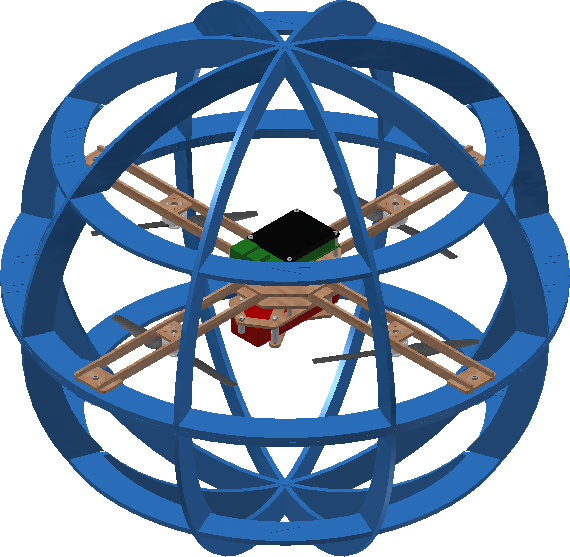
\includegraphics[width=60mm]{image/3DCAD.jpg}
		\caption{作成した3次元CADデータ}
		\label{fig:3DCAD}
	\end{center}
\end{figure}

\begin{table}[htbp]
	\begin{center}
		\caption{物理特性}
		\begin{tabular}{|l|l|r|} \hline
			 & x & 0.607[mm] \\
			重心 & y & -0.266[mm] \\
			 & z & 8.044[mm] \\ \hline
			 & Ix & 82460067.681[g・mm2] \\
			慣性モーメント & Iy & 82647566.473[g・mm2] \\
			 & Iz & 62125193.829[g・mm2] \\ \hline
			 & Ixx & 82508567.214[g・mm2] \\
			 & Iyx & 14332.870[g・mm2] \\
			慣性乗積 & Iyy & 82560633.418[g・mm2] \\
			 & Izx & 115114.862[g・mm2] \\
			 & Izy & 1631241.057[g・mm2] \\
			 & Izz & 62256449.912[g・mm2] \\ \hline
		\end{tabular}
		\label{table:phy}
	\end{center}
\end{table}

\subsubsection{推力特性}
図\ref{fig:thrust-test}のように,はかりにプロペラを付けたモータを固定した実験装置を製作した.
この状態でモータに与えるPWM値を0.05[ms]ずつ上昇させ,PWM値と推力の関係を求める.
後記に記載する最適レギュレータは制御則が線形である必要がある.
そのため実験により得られたグラフからモータの始動から推力の上限に達するまでの範囲を抜き出し,その近似直線をモータの制御式として用いる.
例としてRモータのPWM値と推力の関係を表したものを図\ref{fig:thrust-R}に,その近似直線を表したものを図\ref{fig:thrust-R-kinji}に示す.

\begin{figure}[htbp]
	\begin{center}
		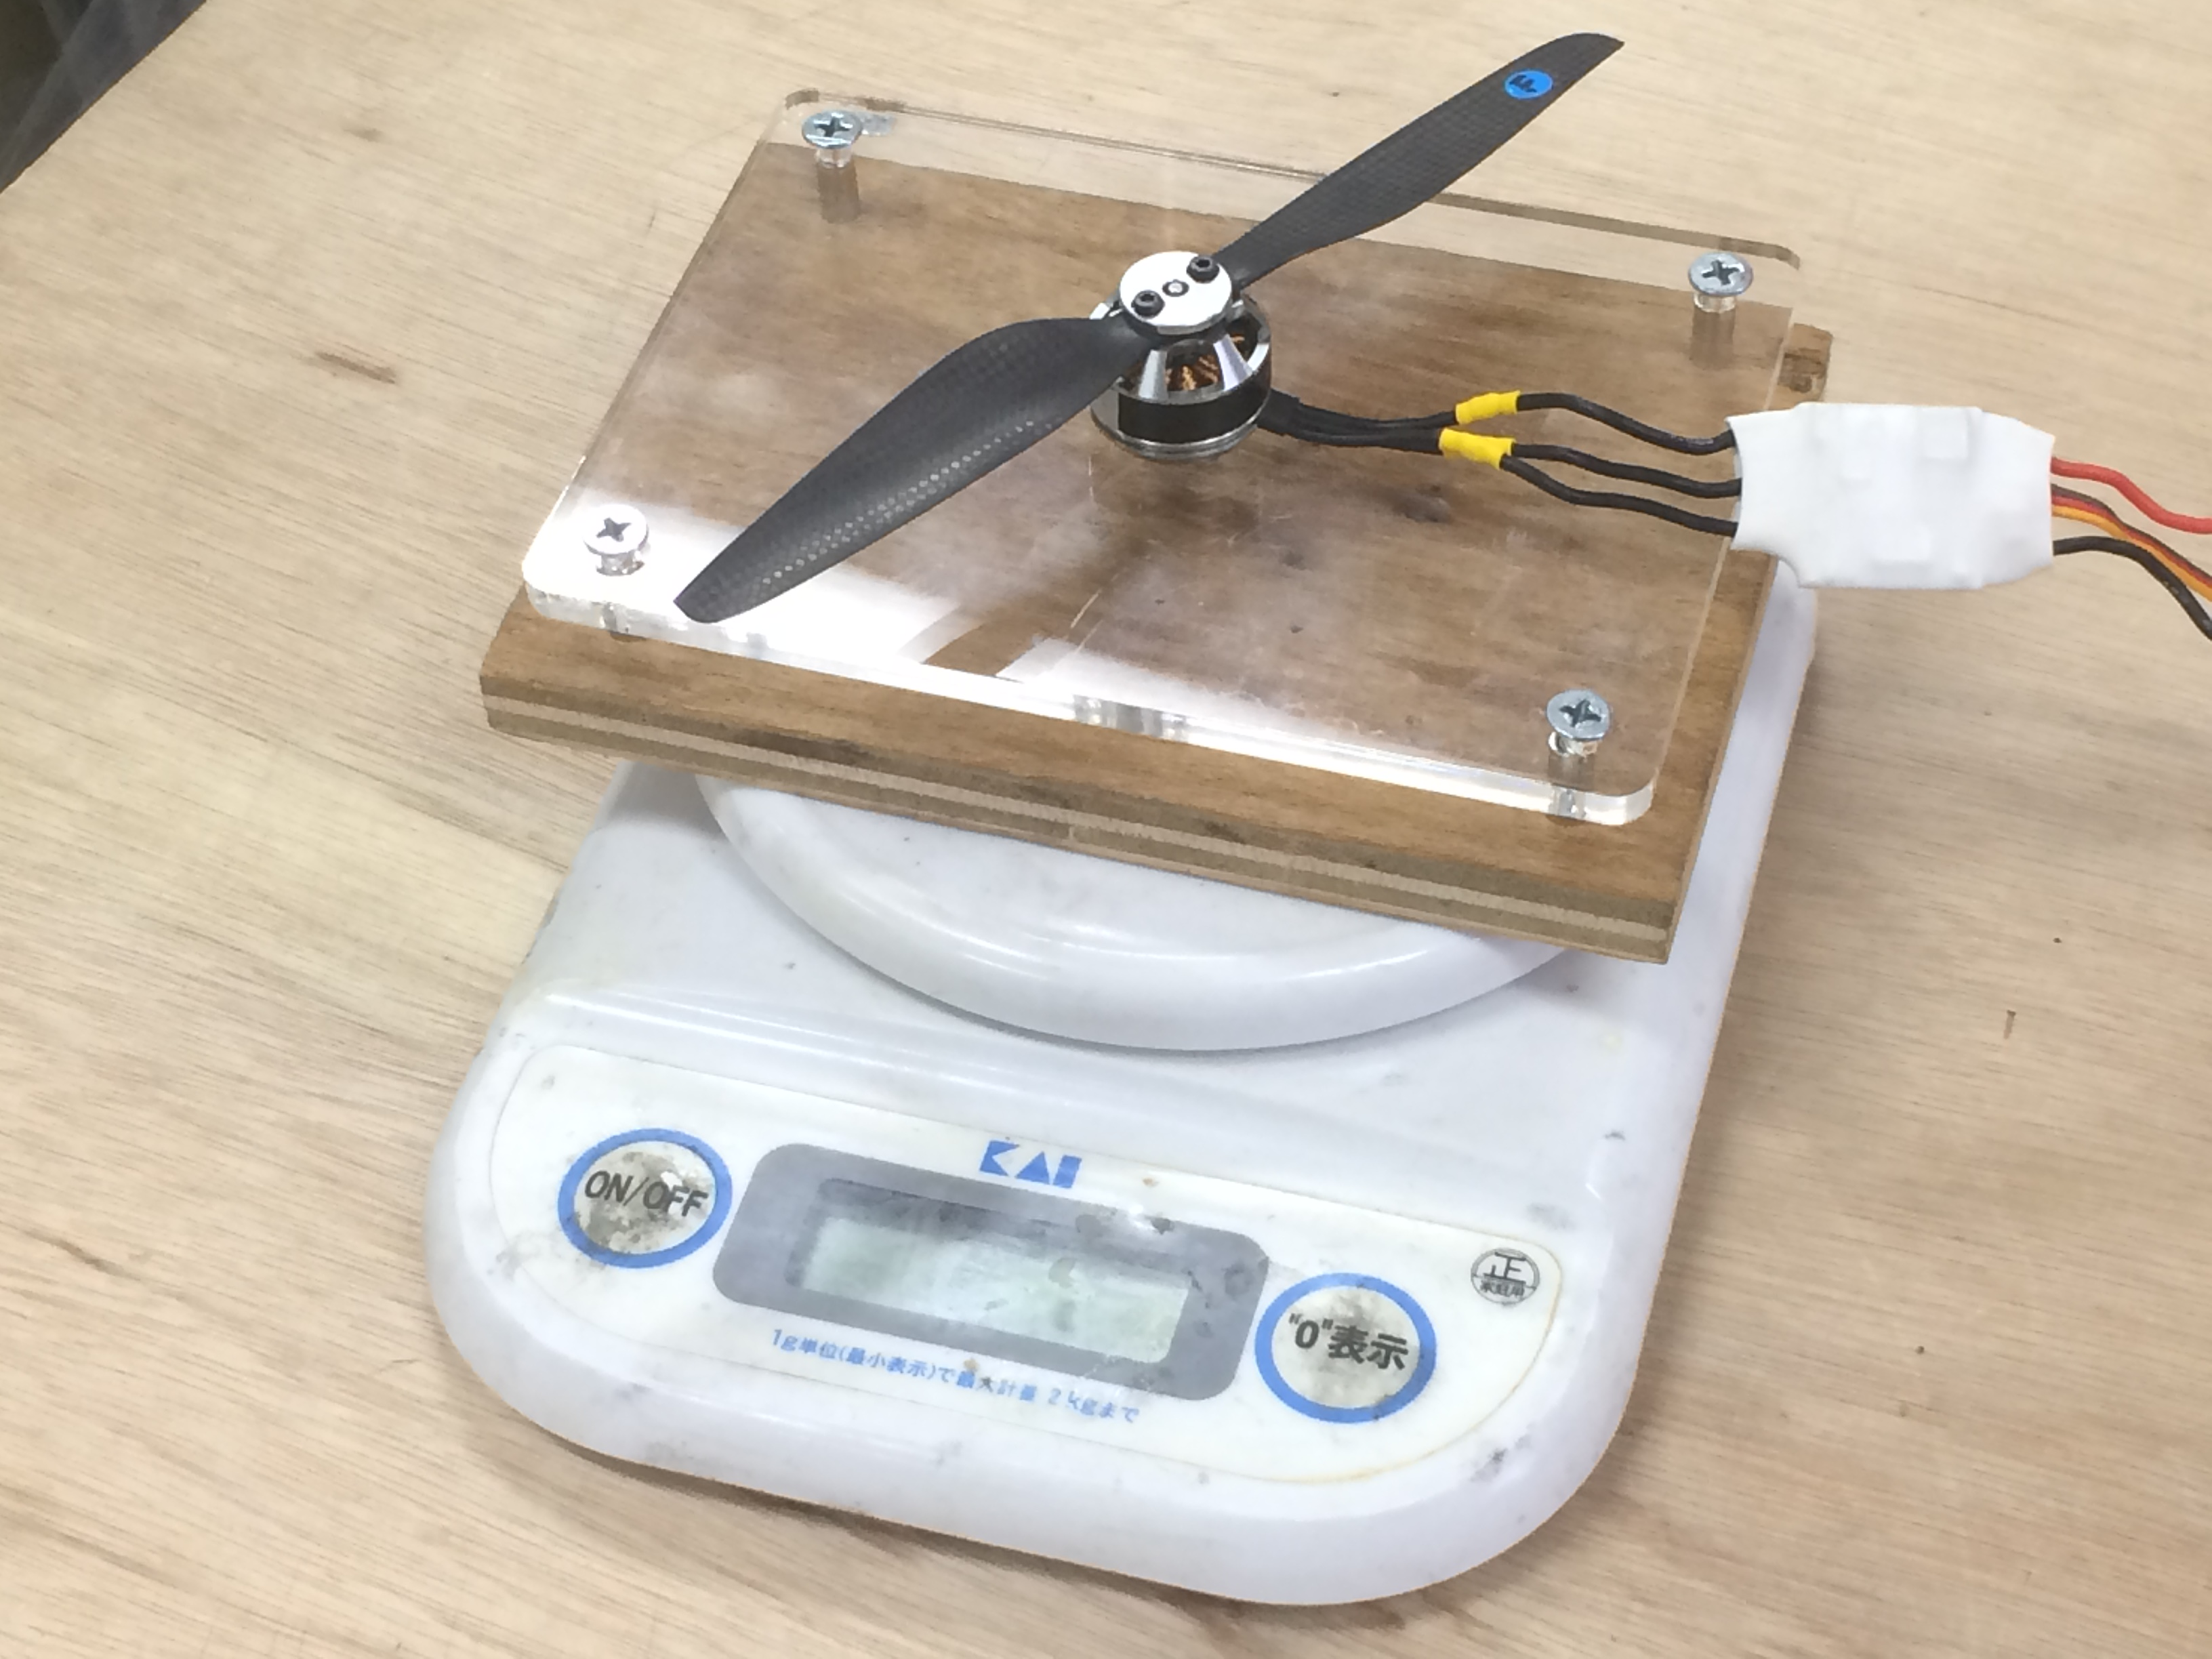
\includegraphics[width=65mm]{image/thrust/thrust-test.jpg}
		\caption{推力特性の確認実験装置}
		\label{fig:thrust-test}
	\end{center}
\end{figure}

\begin{figure}[htbp]
	\begin{center}
		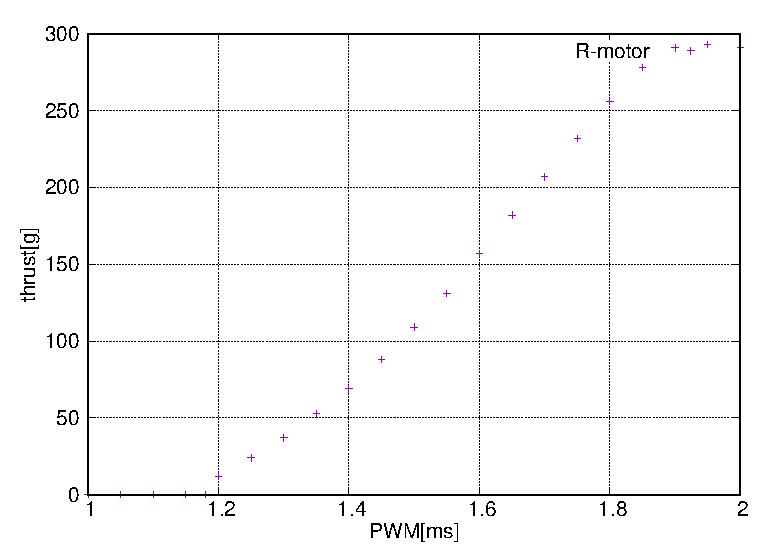
\includegraphics[width=75mm]{image/thrust/thrust-R.eps}
		\caption{RモータのPWM値と推力の関係}
		\label{fig:thrust-R}
	\end{center}
\end{figure}

\begin{figure}[htbp]
	\begin{center}
		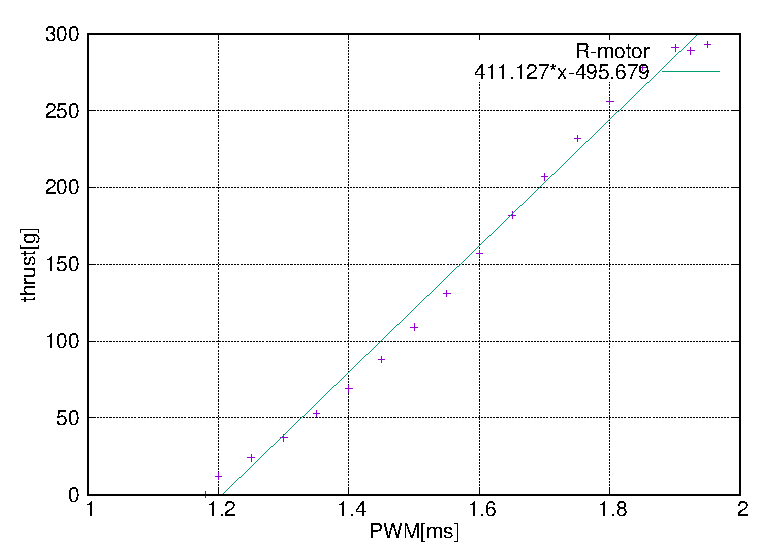
\includegraphics[width=75mm]{image/thrust/thrust-R-kinji.eps}
		\caption{RモータのPWM値と推力の近似直線}
		\label{fig:thrust-R-kinji}
	\end{center}
\end{figure}

\subsubsection{モーメント特性}
図\ref{fig:moment-test}のように,マルチコプターに回転軸を取り付けて吊るした.
この状態で1つのモータで機体が1回転するのにかかる時間を計測する.
こちらも最適レギュレータ使用するので制御則を線形にする.
実験により得られたグラフから機体が1回転するのにかかる時間と◯◯を式(\ref{eq6})に代入し,その近似直線をモータの制御式として用いる.

\begin{equation}
	N = \frac{4J\pi}{t^2}
	\label{eq6}
\end{equation}
 


例としてRモータを回した時の機体が1回転するのにかかる時間を計測したものを図\ref{fig:moment-time-R}に示す.
またモーメントを算出し,PWM値とモーメントの関係とその近似直線を表したものを図\ref{fig:moment-R}に示す.

\begin{figure}[htbp]
	\begin{center}
		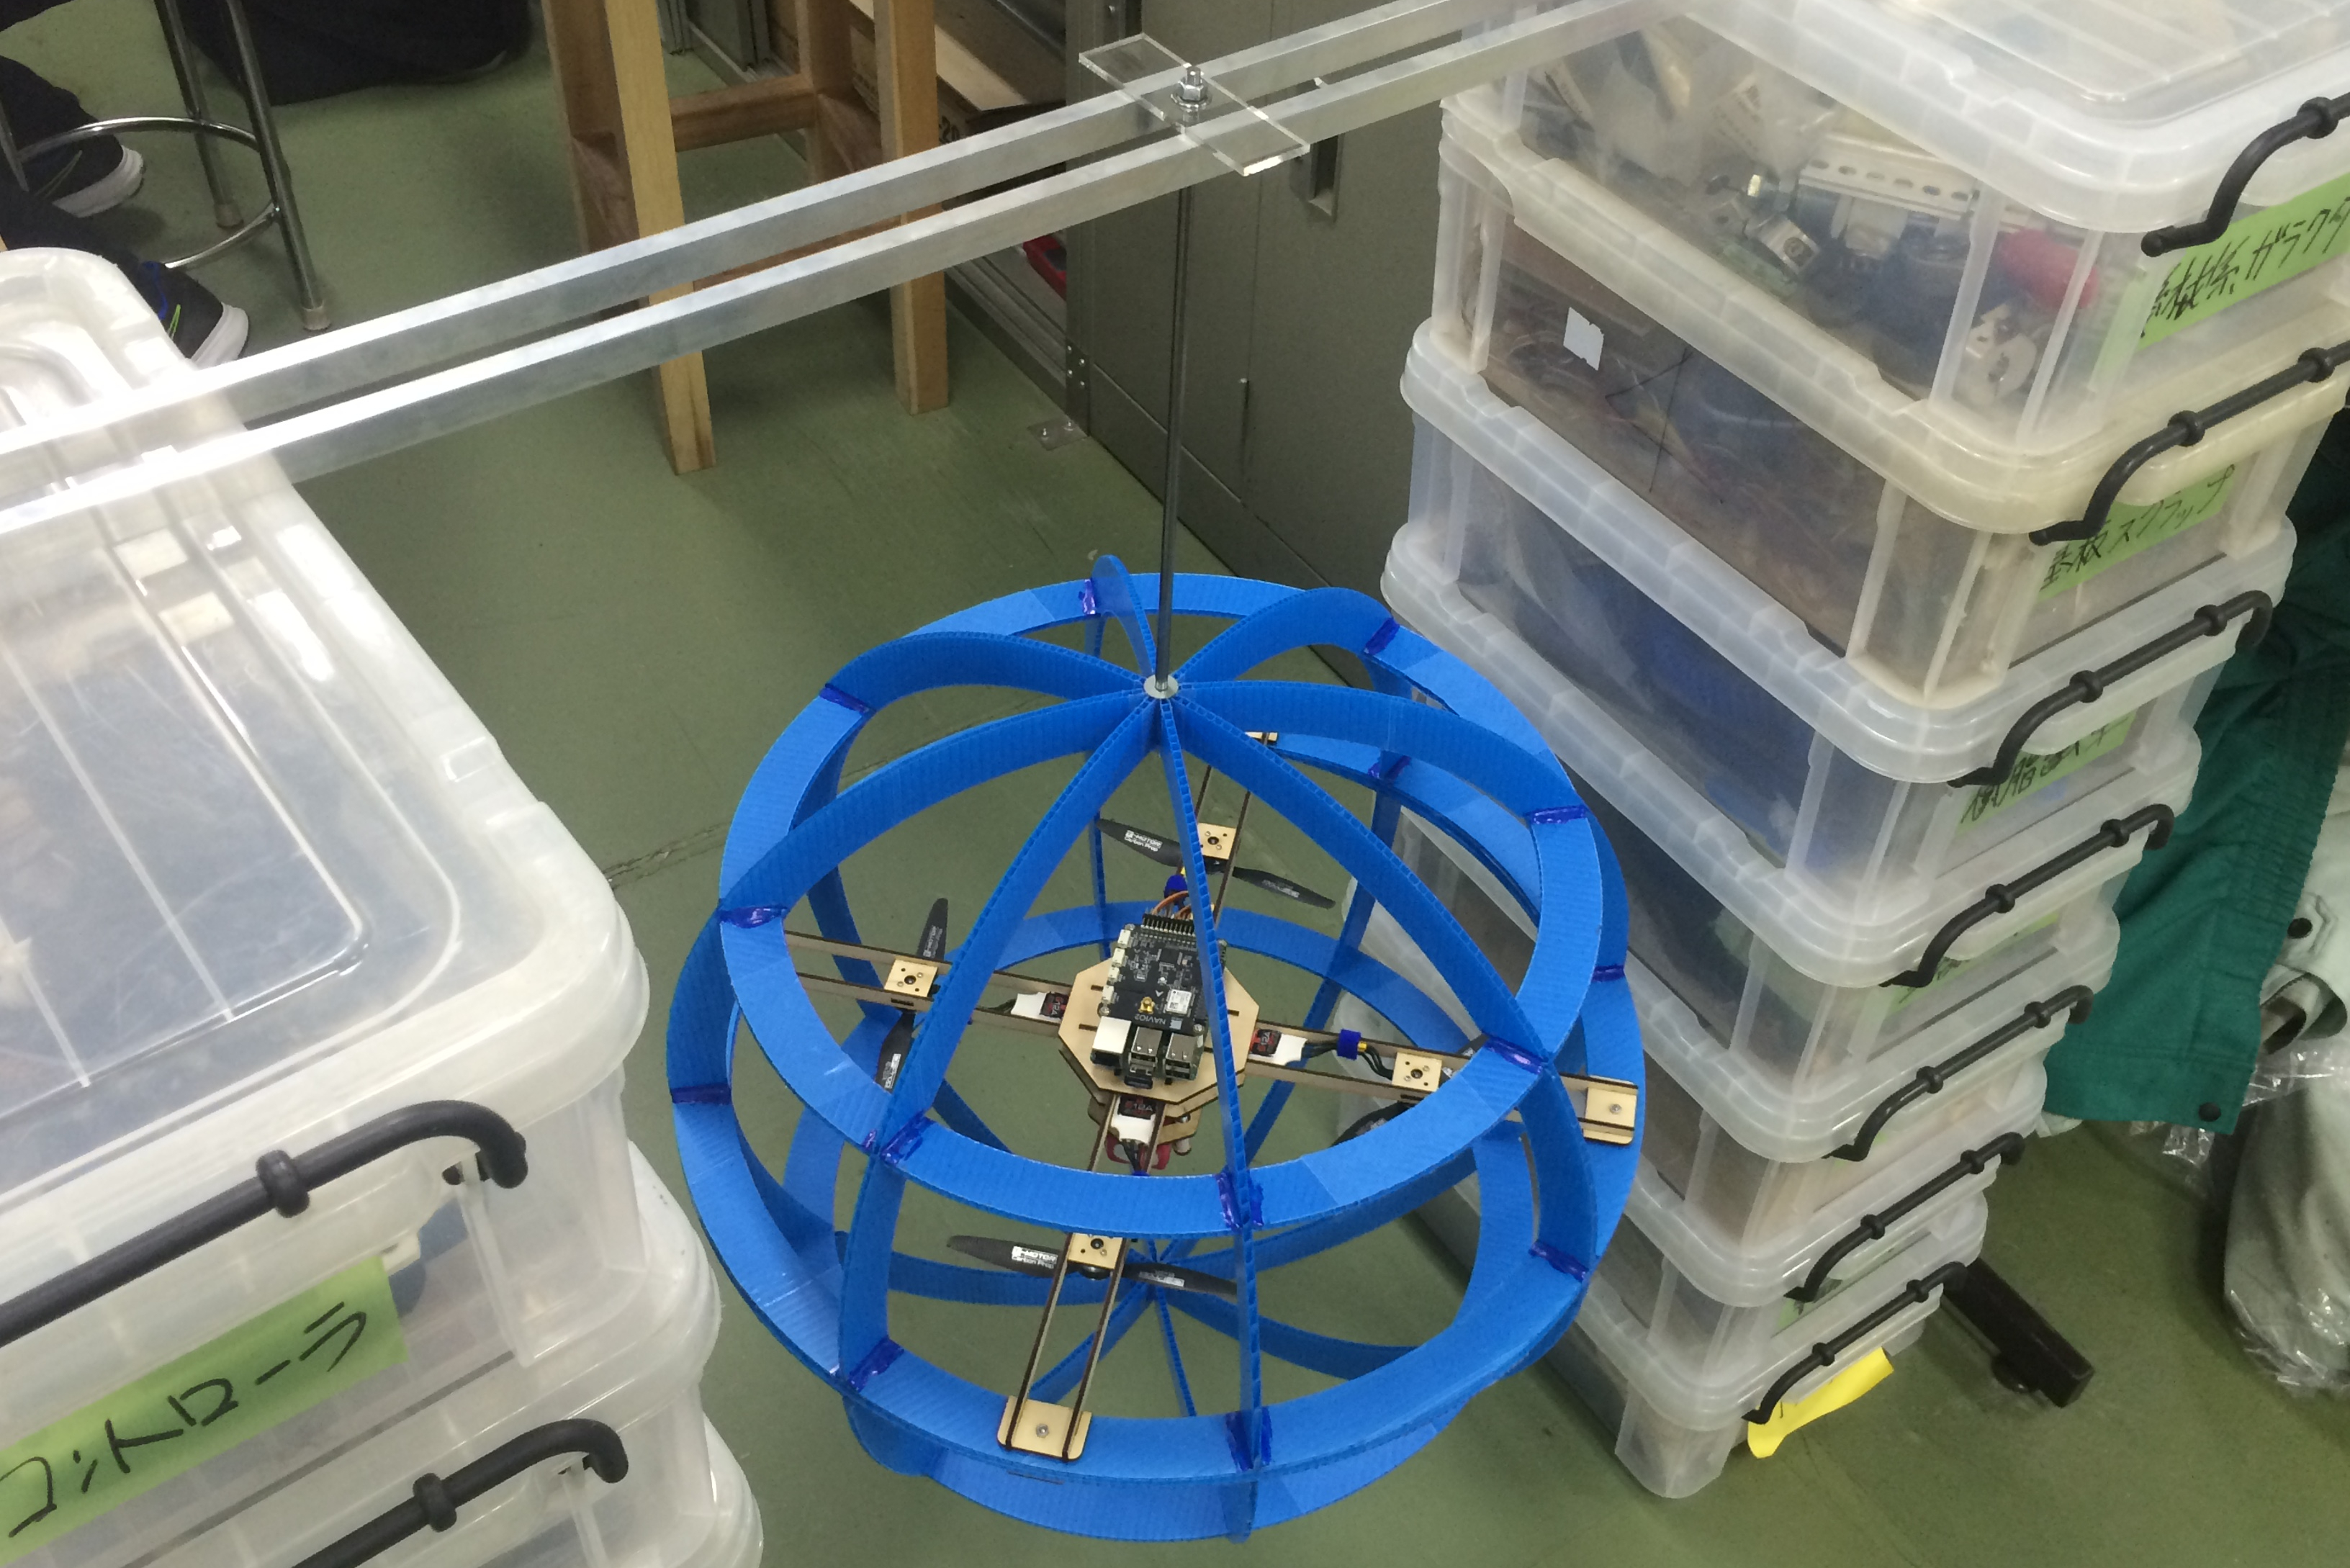
\includegraphics[width=65mm]{image/moment/moment-test.jpg}
		\caption{モーメント確認実験}
		\label{fig:moment-test}
	\end{center}
\end{figure}

\begin{figure}[htbp]
	\begin{center}
		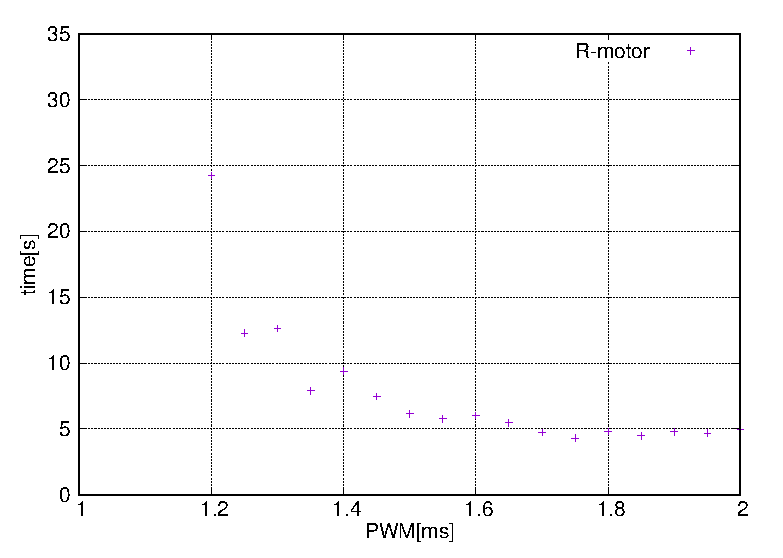
\includegraphics[width=75mm]{image/moment/moment-time-R.eps}
		\caption{RモータのPWM値と1回転にかかる時間の関係}
		\label{fig:moment-time-R}
	\end{center}
\end{figure}

\begin{figure}[htbp]
	\begin{center}
		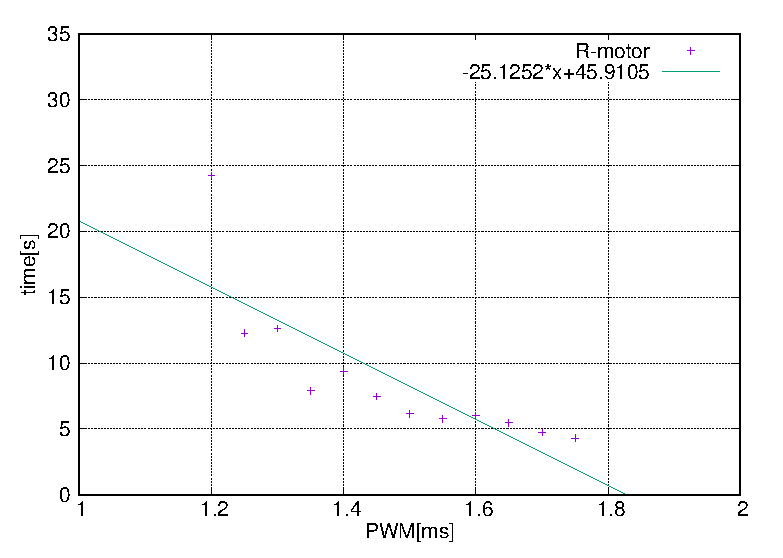
\includegraphics[width=75mm]{image/moment/moment-R.eps}
		\caption{RモータのPWM値とモーメントの関係とその近似直線}
		\label{fig:moment-R}
	\end{center}
\end{figure}

\subsection{ルンゲ・クッタ法を用いた機体のシュミレーション}
上記の実験で運動方程式を解くのに必要な情報が得られたので,ルンゲ・クッタ法を用いて機体のシュミレーションを行った.
以下の表\ref{table:syumi}の条件でシュミレーションを行った.

\begin{table}[htbp]
	\begin{center}
		\caption{シュミレーションの条件}
		\begin{tabular}{|l|l|} \hline
			機体の各変位 & すべて静止の状態と考え0 \\ \hline 
			各種固有値 & 実際の数値を使用 \\ \hline
			モータの状態 & 全てに同じだけの推力を発生 \\ \hline
		\end{tabular}
		\label{table:syumi}
	\end{center}
\end{table}

XYZ方向の移動量のシュミレーション結果を図\ref{fig:UVW}に示す.

\begin{figure}[htbp]
	\begin{center}
		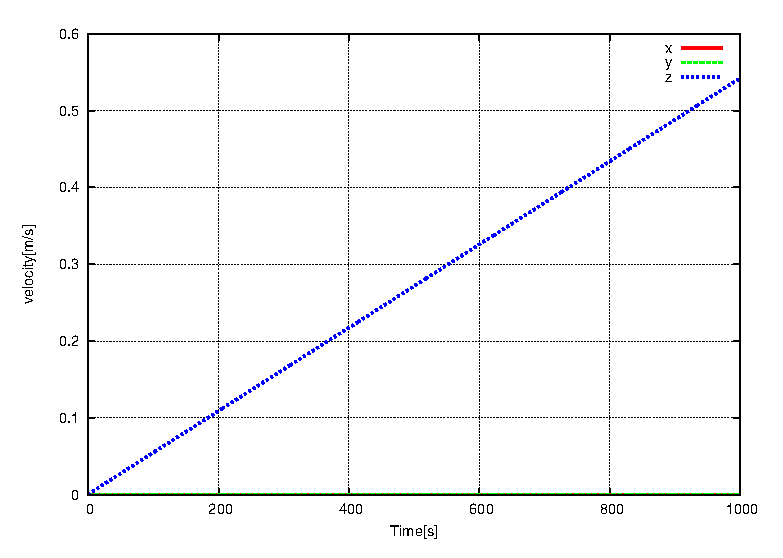
\includegraphics[width=75mm]{image/UVW.eps}
		\caption{各方向の移動量}
		\label{fig:UVW}
	\end{center}
\end{figure}

図\ref{fig:UVW}より,すべてのモータに等しい推力を与えた場合Z方向の移動量だけが増加した.
このように機体の条件を入力することにより機体の動きをシュミレーションすることができる.このシュミレーションと実際の制御時のグラフが正しいかどうかで制御がうまくいっているか確認できる.

\subsection{校正}
制御を正確なものにするため各センサに校正を行った.

\subsubsection{加速度センサ}
各軸の正方向を地面に垂直に向けた状態で複数回データを取り,その平均値をセンサの補正値とする.
センサから出力される値をこの補正値で割ることで校正する.
z軸について,校正前のデータを図\ref{fig:acc-calib-be}に,校正後のデータを図\ref{fig:acc-calib-af}に示す.
加速度の値は校正前からほぼ正しい値を示していたためほとんど変化が見られなかった.

\begin{figure}[htbp]
	\begin{center}
		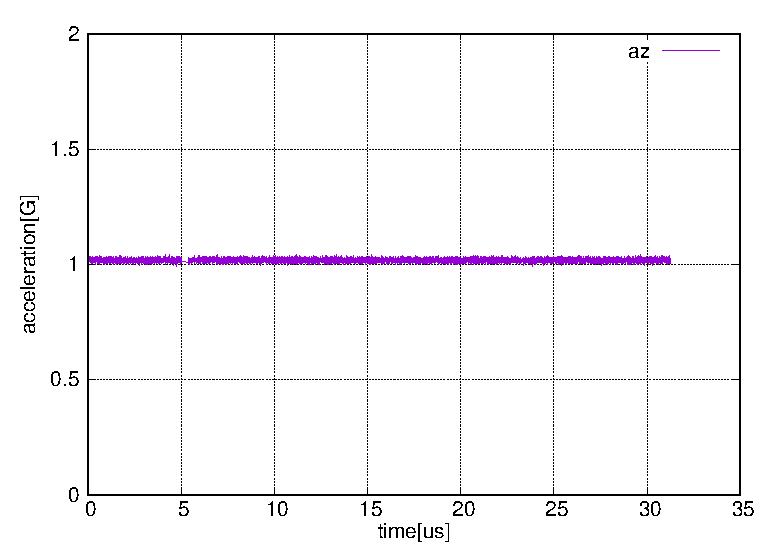
\includegraphics[width=75mm]{image/calibration/acc-calib-be.eps}
		\caption{校正前の加速度データ}
		\label{fig:acc-calib-be}
	\end{center}
\end{figure}

\begin{figure}[htbp]
	\begin{center}
		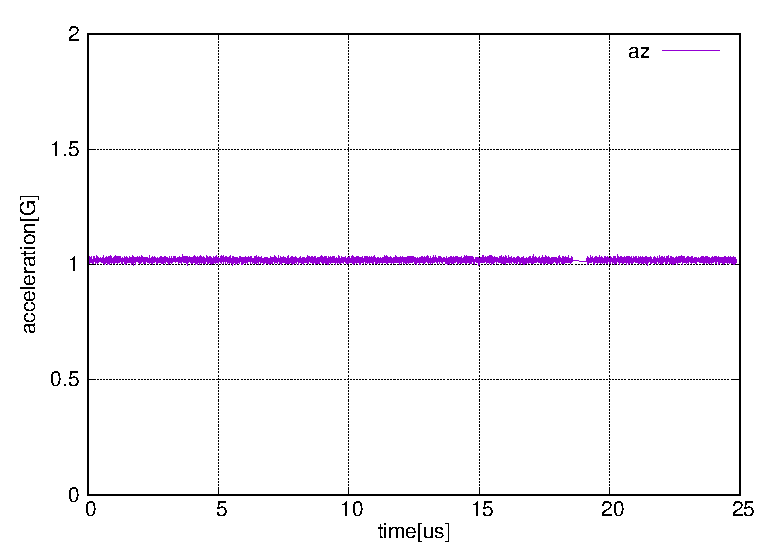
\includegraphics[width=75mm]{image/calibration/acc-calib-af.eps}
		\caption{校正後の加速度データ}
		\label{fig:acc-calib-af}
	\end{center}
\end{figure}

\subsubsection{地磁気センサ}
各軸の正方向を北,南に向けた状態で複数回データを取り,北向きの時のデータの平均値から南向きの時のデータの平均値を引いた値をセンサの補正値とする.
センサから出力された値からこの値を引くことで校正する.
縦軸にx方向の地磁気,横軸にy方向の地磁気をとったグラフを校正前のものを図\ref{fig:mag-calib-be}に,校正後のものを図\ref{fig:mag-calib-af}に示す.
本来x=0,y=0を中心とする正円の点群が得られるのが望ましいが,校正前は中心がずれ,楕円形になっている.
校正後はおおよそ正しいものになった.

\begin{figure}[htbp]
	\begin{center}
		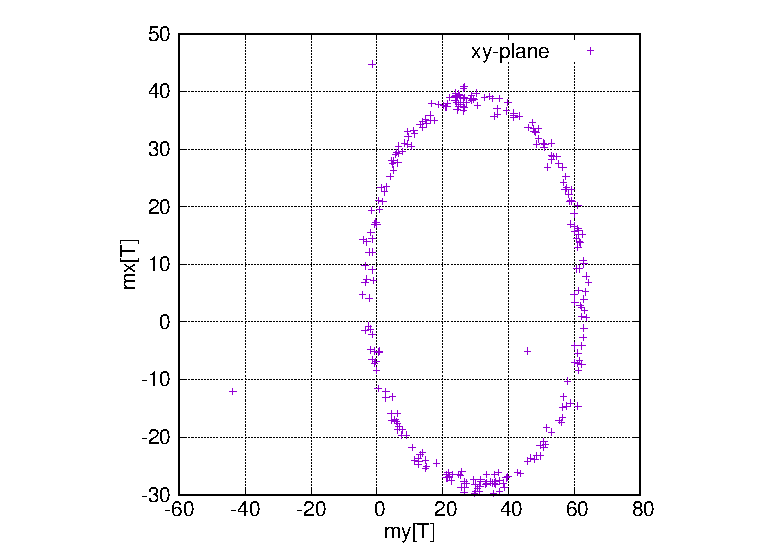
\includegraphics[width=75mm]{image/calibration/mag-calib-be.eps}
		\caption{校正前の地磁気データ}
		\label{fig:mag-calib-be}
	\end{center}
\end{figure}

\begin{figure}[htbp]
	\begin{center}
		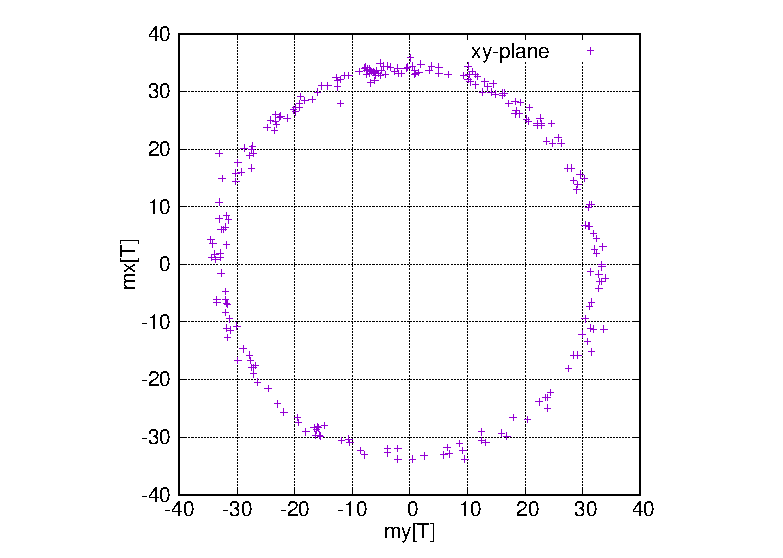
\includegraphics[width=75mm]{image/calibration/mag-calib-af.eps}
		\caption{校正後の地磁気データ}
		\label{fig:mag-calib-af}
	\end{center}
\end{figure}

\section{最適レギュレータ}
以上の結果を用い,最適レギュレータを設計する.

\subsection{最適レギュレータについて}
%解いた運動方程式を線形化し,その線形化したモデルに最適レギュレータを設計した.
%最適レギュレータはセンサから得られた機体の各変位量を常にフィードバックし,その変位量が0になるよう制御して機体の状態を安定させる制御器である.

最適レギュレータとは,評価関数を設け,それを最小とするように状態フィードバックによる最適制御入力を決定する設計法について以下に述べる.可制御で線形な時不定システムの式(\ref{eq7})

\begin{equation}
	\dot{x}(t) = Ax(t)+Bu(t)
	\label{eq7}
\end{equation}

のもとで,ある評価関数を最小にする制御則が線形な状態フィードバック制御則となるため,評価関数は評価関数を以下の2次形式の式(\ref{eq8})にする必要がある.

\begin{equation}
	J = \int^{t_f}_0 [x^T(t)Qx(t)+u^T(t)Ru(t)]dt
	\label{eq8}
\end{equation}

ここで,制御目的の重み行列Q(n×n)は非負定な対称行列,制御入力の重み行列R(m×m)は正定対称行列とする.\cite{regyu}

\subsection{最適レギュレータの結果}
最適レギュレータにより,球体カバーを取り付けた状態での離陸が可能となった.


\chapter{おわりに}


\chapter*{謝辞}
\addcontentsline{toc}{chapter}{謝辞}
本論文作成にあたりテーマの決定,研究の考え方,方法のまとめ方など全てにおいて長期にわたって厳しくも熱意のあるご指導,ご鞭撻していただいた,伊藤恒平教授に厚く御礼申し上げます.


特に分析においても論文の書き方においても論文を何度も読んでいただき,指導していただいた伊藤恒平教授に大変ご苦労をかけてしまいましたことにも心よりお詫び申し上げたいです.


同級生のメンバーには論文の作成,修正にご協力いただき心より感謝しております.
その他、助けていただいた多くの皆様に心から感謝しております.ありがとうございました.


\chapter*{付録}
\addcontentsline{toc}{chapter}{付録}

\section{レーザー加工機}
機体,球体の製作にはレーザー加工機を使用するため,レーザー加工機について説明する.
レーザー加工機は"プリンター"である.

\subsection{加工可能な材料}
アクリルなどのプラスチックや木,紙,コルク材などの材質が加工可能である.
ただし塩ビなどの一部材質では、加工時に有毒ガスが発生するため加工不可である.
大きさは460mm×640mm,厚さ約5mm程度まで加工可能である.

\subsection{加工データ}
加工データは主に加工機横に設置されているパソコンでCorelDRAWというペイントソフトを用いて作成する.
dxf形式のデータやpng,jpgなどの画像も読み込むことができる.

\subsection{加工時の設定}
加工時には速度,レーザーの出力,DPI(Dot per inch)などが設定可能である.
この値は材質によって異なる.
基準値は説明書に記載されているが,実際に切ってみて調整を行うほうが良い.

\section{ソースコード}
実際に使用したソースコードを以下に示す.


\end{document}

